\documentclass[10pt,a4paper]{article}
\usepackage[utf8]{inputenc}
\usepackage{graphicx}
\def\Pr{\mathop{\rm Pr}}
\usepackage[landscape,margin=1cm]{geometry}
\usepackage[english]{babel}
\usepackage{tikz}
%\setmainfont{Rubik}[Scale=1.0]

\usetikzlibrary{arrows,snakes,backgrounds,shapes.geometric}
\title{Neuromatch Academy Pre-Requisite Refresher - Summary Sheet}
\author{Neuromatch}
%\date{July 2019}
\usepackage[default]{raleway}
\usepackage{fontawesome}
\usepackage[T1]{fontenc}

\usepackage{hyperref}
\usepackage{enumitem}
\usepackage{lipsum}

\usepackage{xcolor}
\definecolor{customcolor}{HTML}{616AC5}
\definecolor{alert}{HTML}{CD5C5C}
\definecolor{w3schools}{HTML}{4CAF50}
\definecolor{subbox}{gray}{0.60}
\definecolor{codecolor}{HTML}{FFC300}
\colorlet{xx}{customcolor}


%--------------------------Editor mode.

\usepackage
[citestyle=authoryear,
sorting=nty,	  		%Sorts bibliography by year, name, title
autocite=footnote, 		%Autocite command generates footnotes
autolang=hyphen, 		
mincrossrefs=1, 	
backend=biber]
{biblatex}

\DeclareFieldFormat{postnote}{#1}
\DeclareFieldFormat{multipostnote}{#1}
\DeclareAutoCiteCommand{footnote}[f]{\footcite}{\footcites}

\bibliography{literature}
%----------------------------------------
%--------------------------------------------------------------------------------
\usepackage{tcolorbox}

\tcbuselibrary{most,listingsutf8,minted}

\tcbset{tcbox width=auto,left=1mm,top=1mm,bottom=1mm,
right=1mm,boxsep=1mm,middle=1pt}

\newenvironment{mycolorbox}[2]{%
\begin{tcolorbox}[grow to left by=-1em,grow to right by=-1em,capture=minipage,fonttitle=\large\bfseries, enhanced jigsaw,boxsep=1mm,colback=#1!30!white,on line,tcbox width=auto, toptitle=0mm,colframe=#2,opacityback=0.7,nobeforeafter,title=#2]%
}{\end{tcolorbox}\\[0.2em]}

\newenvironment{subbox}[2]{%
\begin{tcolorbox}[capture=minipage,fonttitle=\scriptsize\bfseries, enhanced jigsaw,boxsep=1mm,colback=#1!30!white,on line,tcbox width=auto,left=0.3em,top=1mm, toptitle=0mm,colframe=#1,opacityback=0.7,nobeforeafter,title=#2]\footnotesize %
}{\normalsize\end{tcolorbox}\vspace{0.1em}}

\newenvironment{multibox}[1]{%
\begin{tcbraster}[raster columns=#1,raster equal height,nobeforeafter,raster column skip=1em,raster left skip=1em,raster right skip=1em]}{\end{tcbraster}}

\newenvironment{textbox}[1]{\begin{mycolorbox}{customcolor}{#1}}{\end{mycolorbox}}

%-------------------------------
\newtcblisting{codebox}[2]{colback=codecolor!5,colframe=codecolor!80!black,listing only, 
minted options={numbers=left,style=tcblatex,fontsize=\normalsize,breaklines,autogobble,linenos,numbersep=1mm},
left=5mm,enhanced,
title=#2, fonttitle=\bfseries,
listing engine=minted,minted language=#1}

%--------------------------------------------------------------------------------
\newcommand{\punkti}{~\lbrack\dots\rbrack~}

\renewenvironment{quote}
               {\list{\faQuoteLeft\phantom{ }}{\rightmargin\leftmargin}%
                \item\relax\scriptsize\ignorespaces}
               {\unskip\unskip\phantom{xx}\faQuoteRight\endlist}
               

%--------------------------------------------------------------------------------
\newcommand{\bgupper}[3]{\colorbox{#1}{\color{#2}\huge\bfseries\MakeUppercase{#3}}}
\newcommand{\bg}[3]{\colorbox{#1}{\bfseries\color{#2}#3}}

\newcommand{\mycommand}[2]{{\ttfamily\detokenize{#1}}~\dotfill{}~{\footnotesize #2}\\}
\newcommand{\sep}{{\scriptsize~\faCircle{ }~}}


\newcommand{\bggreen}[1]{\medskip\bgupper{w3schools}{black}{#1}\\[0.5em]}
\newcommand{\green}[1]{\smallskip\bg{w3schools}{white}{#1}\\}
\newcommand{\red}[1]{\smallskip\bg{alert}{white}{#1}\\}

\usepackage{multicol}
\setlength{\columnsep}{30pt}

\setlength{\parindent}{0pt}
\pagestyle{empty}

\usepackage{csquotes}

\newcommand{\loremipsum}{Lorem ipsum dolor sit amet.}

\clearpage
%\defaultfontfeatures{ Scale=MatchUppercase, Ligatures=TeX }
%\setmathfont{Fira Math}
%\setmathfont{Rubik}[range=up]
%--------------------------------------------------------------------------------
\begin{document}


%\section{Data Type}

\includegraphics[scale=0.03]{Figures/NMACN.png}\href{https://compneuro.neuromatch.io/tutorials/intro.html}{\textbf{\Huge{Neuromatch Academy: Linear Systems - Summary Sheet}}\footnote{’t Hart et al., (2022). Neuromatch Academy: a 3-week, online summer school in computational neuroscience. Journal of Open Source Education, 5(49), 118. https://doi.org/10.21105/jose.00118}}
%$\subsection*{Cheat Sheet}
\small
\begin{multicols}{3}
%\scriptsize
%\pagecolor{black}

\let\clearpage\relax
\begin{textbox}{\href{https://compneuro.neuromatch.io/tutorials/W2D2_LinearSystems/student/W2D2_Tutorial1.html}{Linear Dynamical Systems }   }
\begin{subbox}{subbox}{One-dimensional Differential Equations}
\scriptsize
Differential equations are equations that express the \textbf{rate of change} of the state variable $x$. One typically describes this rate of change using the derivative of $x$ with respect to time ($dx/dt$) on the left hand side of the differential equation:

$$\frac{dx}{dt} = f(x)$$

A common notational short-hand is to write $\dot{x}$ for $\frac{dx}{dt}$. The dot means "the derivative with respect to time".
We can simulate an ordinary differential equation by approximating or modeling time as a discrete list of time steps $t_0, t_1, t_2, \dots$, such that $t_{i+1}=t_i+dt$. We can get the small change $dx$ over a small duration $dt$ of time from the definition of the differential:
\begin{eqnarray}
  \dot x &=& \frac{dx}{dt} \\
  dx     &=& \dot x\, dt  
\end{eqnarray}
So, at each time step $t_i$, we compute a value of $x$, $x(t_i)$, as the sum of the value of $x$ at the previous time step, $x(t_{i-1})$ and a small change $dx=\dot x\,dt$:

$$x(t_i)=x(t_{i-1})+\dot x(t_{i-1}) dt$$
This very simple integration scheme, known as \textbf{forward Euler integration}, works well if $dt$ is small and the ordinary differential equation is simple.

The solution of the differential equation $\dot{x} = a x$ using forward Euler integration is: 

\centering
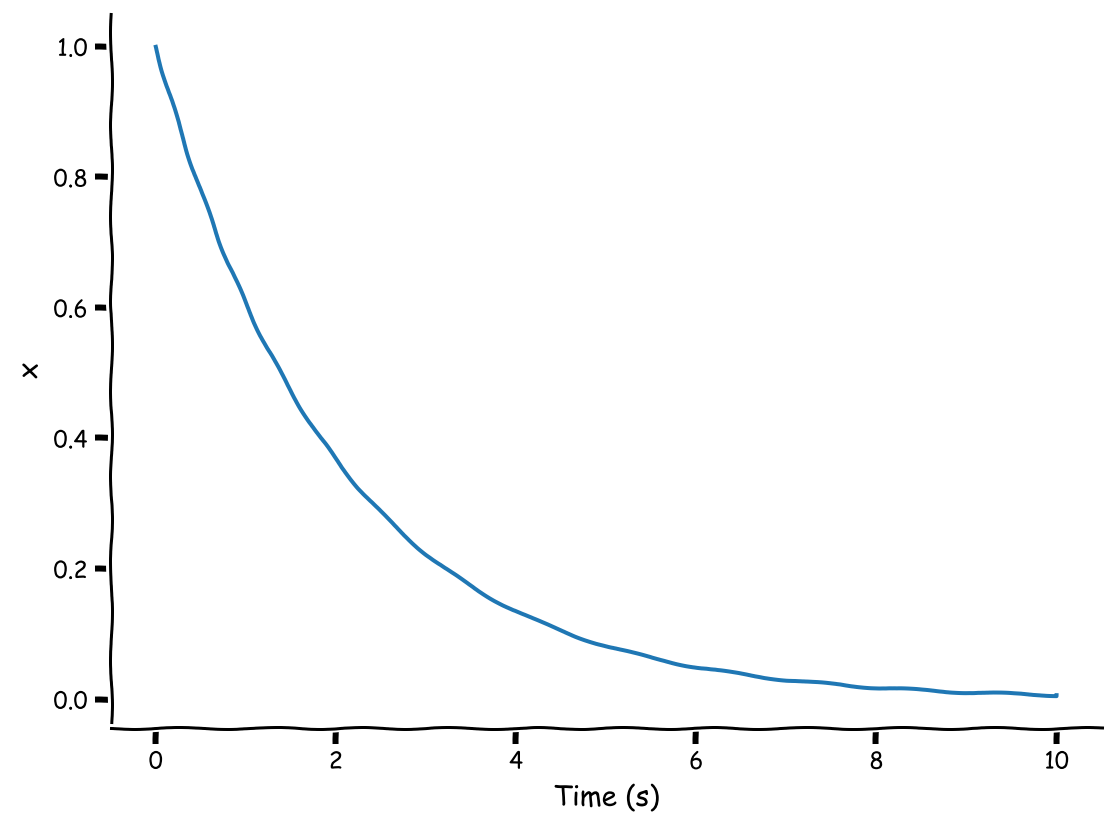
\includegraphics[scale=0.15]{Figures/LS/LSFigure1.png}
\end{subbox}
\end{textbox}
%%%%%%%%%%%%%%%%%%%%%%%%% 
%%%%%%%%%%%%%%%%%%%%%%%%%
\begin{textbox}{\href{https://compneuro.neuromatch.io/tutorials/W2D2_LinearSystems/student/W2D2_Tutorial1.html}{Linear Dynamical Systems } }
\begin{subbox}{subbox}{Multi-Dimensional Dynamics}
\scriptsize
Adding one additional variable (or dimension) adds more variety of behaviors. Additional variables are useful in modeling the dynamics of more complex systems with richer behaviors, such as systems of multiple neurons. We can write such a system using two linear ordinary differential equations:

\begin{eqnarray}
  \dot{x}_1 &=& {a}_{11} x_1 \\
  \dot{x}_2 &=& {a}_{22} x_2 
\end{eqnarray}

So far, this system consists of two variables (e.g. neurons) in isolation. To make things interesting, we can add interaction terms:

\begin{eqnarray}
  \dot{x}_1 &=& {a}_{11} x_1 + {a}_{12} x_2 \\
  \dot{x}_2 &=& {a}_{21} x_1 + {a}_{22} x_2 
\end{eqnarray}

We can write the two equations that describe our system as one (vector-valued) linear ordinary differential equation:

$$\dot{\mathbf{x}} = \mathbf{A} \mathbf{x}$$

For two-dimensional systems, $\mathbf{x}$ is a vector with 2 elements ($x_1$ and $x_2$) and $\mathbf{A}$ is a $2 \times 2$ matrix with 
$$\mathbf{A}=
\begin{pmatrix}
 a_{11} & a_{12} \\
 a_{21} & a_{22} 
\end{pmatrix}.
$$
\centering
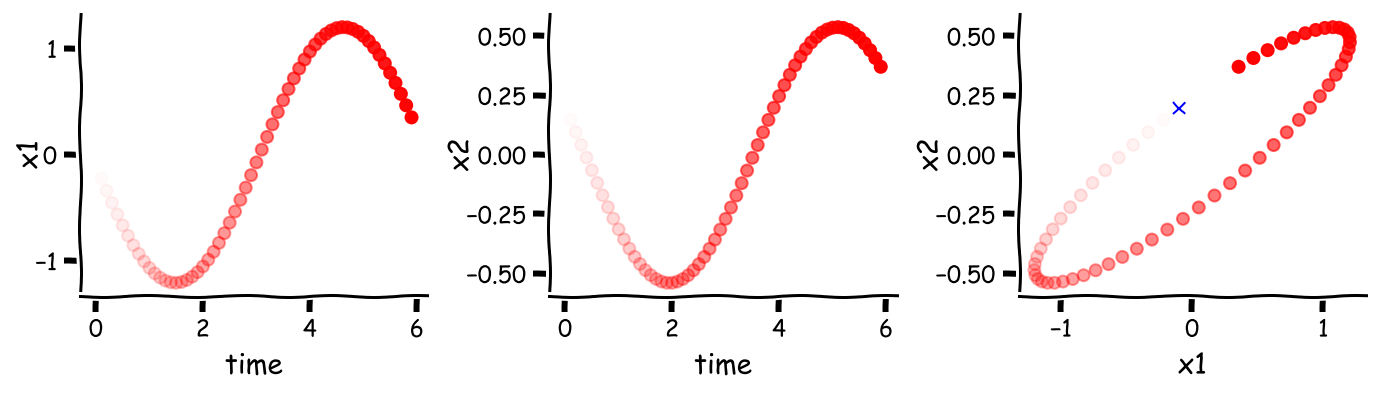
\includegraphics[scale=0.14]{Figures/LS/LSFigure2.png}

\end{subbox}

\end{textbox}
%%%%%%%%%%%%%%%%%%%%%%%%% 
%%%%%%%%%%%%%%%%%%%%%%%%%
\begin{textbox}{\href{https://compneuro.neuromatch.io/tutorials/W2D2_LinearSystems/student/W2D2_Tutorial1.html}{Linear Dynamical Systems } }
\begin{subbox}{subbox}{Stream Plots}
\scriptsize
It's a bit tedious to plot trajectories one initial condition at a time!

Fortunately, to get an overview of how a grid of initial conditions affect trajectories of a system, we can use a \textit{stream plot}. 

We can think of a initial condition ${\bf x}_0=(x_{1_0},x_{2_0})$  as coordinates for a position in a space. For a 2x2 matrix $\bf A$, a stream plot computes at each position $\bf x$ a small arrow that indicates $\bf Ax$ and then connects the small arrows to form \textit{stream lines}. Remember from the beginning of this tutorial that $\dot {\bf x} = \bf Ax$ is the rate of change of $\bf x$. So the stream lines indicate how a system changes. If you are interested in a particular initial condition ${\bf x}_0$, just find the corresponding position in the stream plot. The stream line that goes through that point in the stream plot indicates ${\bf x}(t)$.

Using some helper functions, we show the stream plots for each option of A that you examined in the earlier interactive demo. We included the eigenvectors of $\bf A$ as a red line (1st eigenvalue) and a blue line (2nd eigenvalue) in the stream plots.

\centering
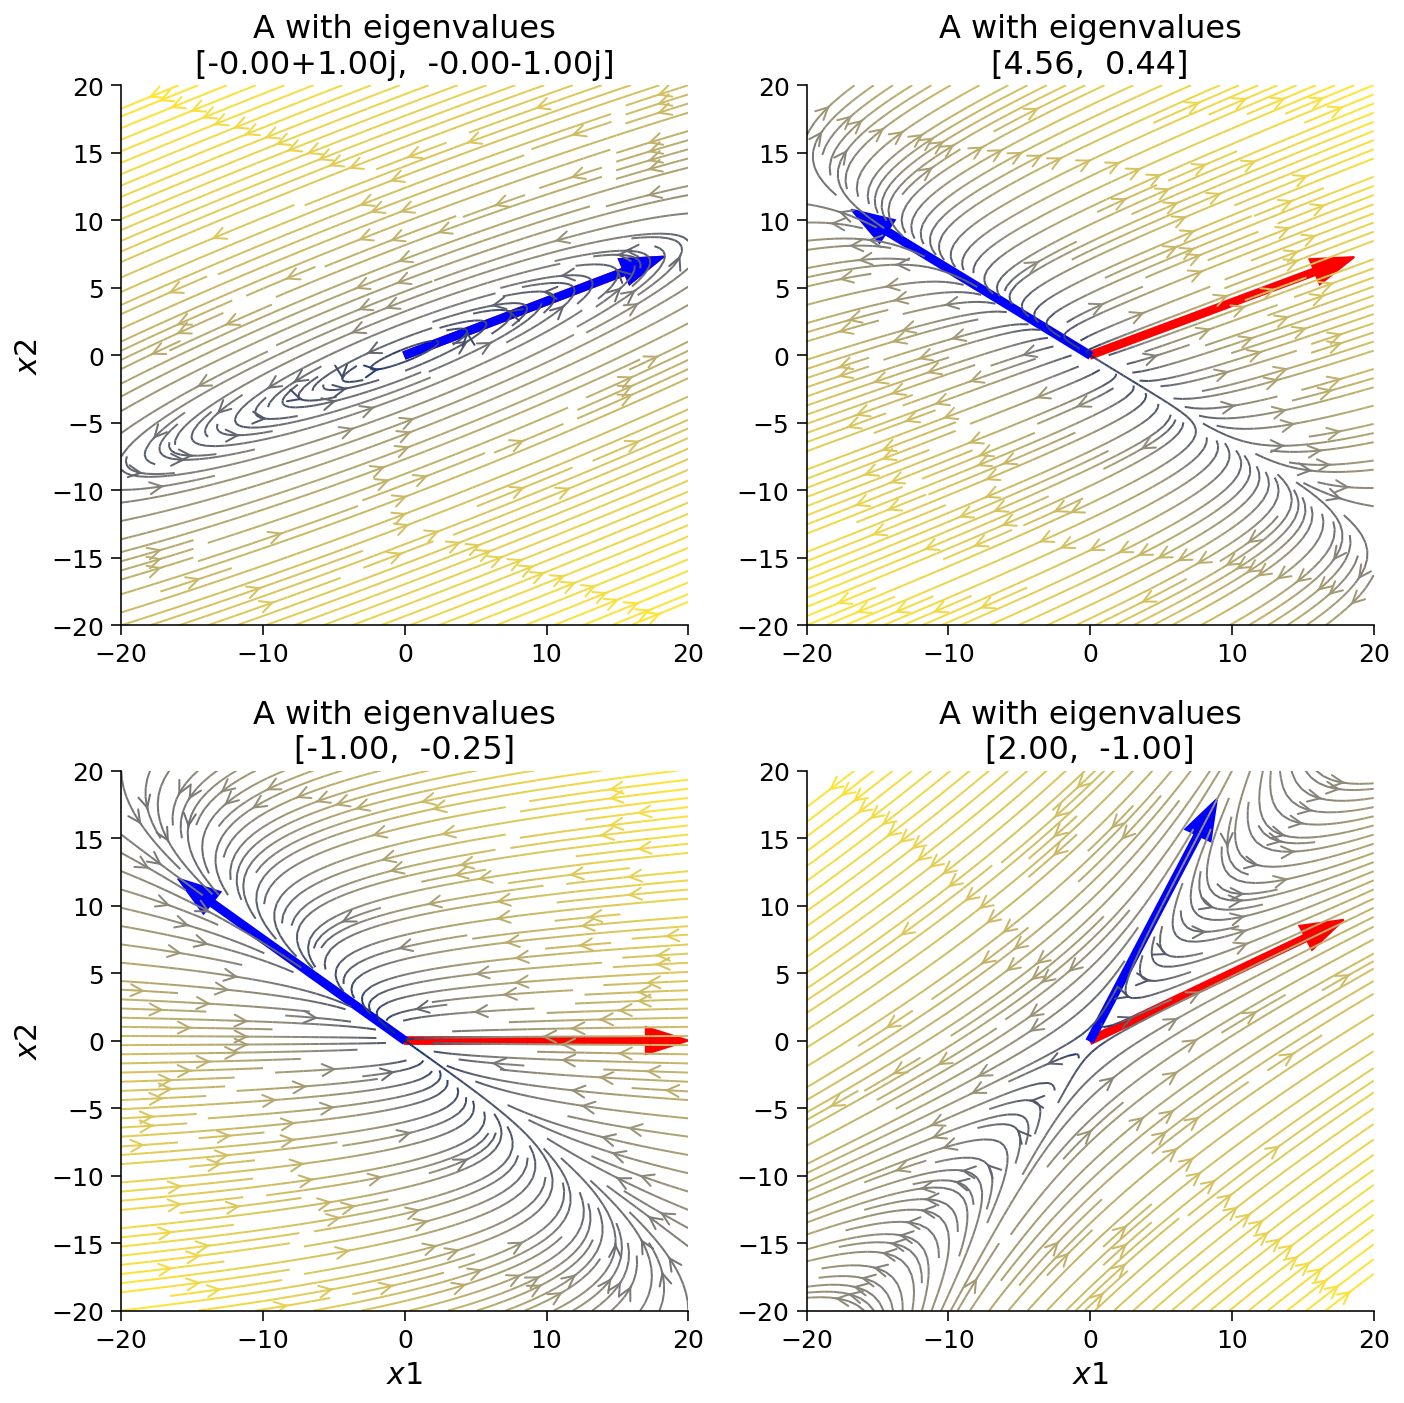
\includegraphics[scale=0.25]{Figures/LS/LSFigure3.png}
\end{subbox}
\end{textbox}
%%%%%%%%%%%%%%%%%%%%%%%%% 
%%%%%%%%%%%%%%%%%%%%%%%%%
\begin{textbox}{\href{https://colab.research.google.com/github/NeuromatchAcademy/course-content/blob/master/tutorials/W2D2_LinearSystems/student/W2D2_Tutorial2.ipynb}{Markov Processes }   }
\begin{subbox}{subbox}{  Introduction }

\scriptsize

We will now look at \textbf{probabilistic} dynamical systems. You may sometimes hear these systems called \textit{stochastic}. In a probabilistic process, elements of randomness are involved. Every time you observe some probabilistic dynamical system, starting from the same initial conditions, the outcome will likely be different. Put another way, dynamical systems that involve probability will incorporate random variations in their behavior. 

For some probabilistic dynamical systems, the differential equations express a relationship between $\dot{x}$ and $x$ at every time $t$, so that the direction of $x$ at every time depends entirely on the value of $x$. Said a different way, knowledge of the value of the state variables $x$ at time t is all the information needed to determine $\dot{x}$ and therefore $x$ at the next time.

This property that the present state entirely determines the transition to the next state  is what defines a \textbf{Markov process} and systems obeying this property can be described as \textbf{Markovian}.


\end{subbox}
\begin{subbox}{subbox}{ Telegraph Process}

\scriptsize

Let's consider a Markov process with two states, where switches between each two states are probabilistic (known as a telegraph process). To be concrete, let's say we are modeling an \textit{ion channel in a neuron that can be in one of two states: Closed (0) or Open (1)}. 

If the ion channel is Closed, it may transition to the Open state with probability $P(0 \rightarrow 1 | x = 0) = \mu_{c2o}$. Likewise, If the ion channel is Open, it transitions to Closed with probability $P(1 \rightarrow 0 | x=1) = \mu_{o2c}$.

We simulate the process of changing states as a Poisson process. The Poisson process is a way to model discrete events where the average time between event occurrences is known but the exact time of some event is not known. Importantly, the Poisson process dictates the following points: 

1. The probability of some event occurring is independent from all other events.

2. The average rate of events within a given time period is constant.

3. Two events cannot occur at the same moment. Our ion channel can either be in an open or closed state, but not both simultaneously. 

In the plot below, we will use the Poisson process to model the state of our ion channel at all points $t$ within the total simulation time $T$. We also track at which times throughout the simulation the state makes a switch. 

\centering
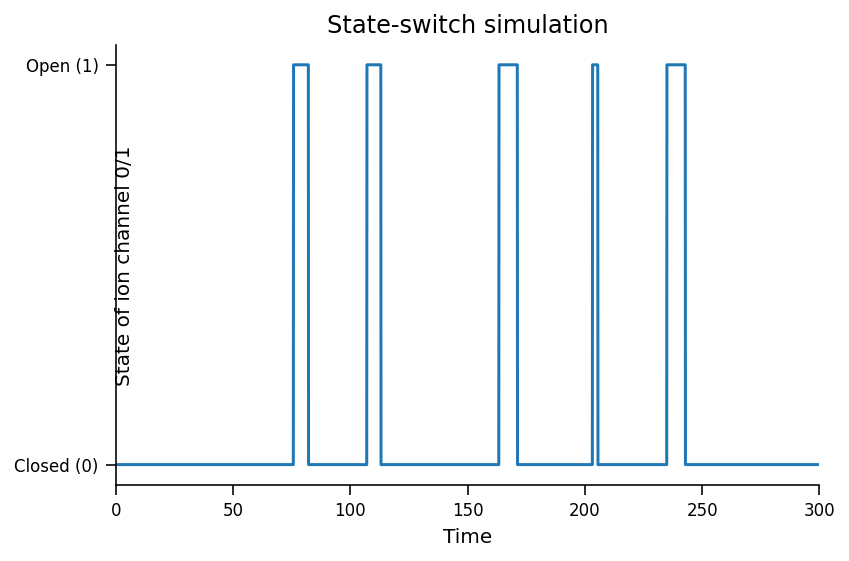
\includegraphics[scale=0.25]{Figures/LS/MC_Figure1.png}

\end{subbox}
\end{textbox}
%%%%%%%%%%%%%%%%%%%%%%%%% 
%%%%%%%%%%%%%%%%%%%%%%%%%
%%%%%%%%%%%%%%%%%%%%%%%%% 
%%%%%%%%%%%%%%%%%%%%%%%%%
\begin{textbox}{\href{https://colab.research.google.com/github/NeuromatchAcademy/course-content/blob/master/tutorials/W2D2_LinearSystems/student/W2D2_Tutorial2.ipynb}{Markov Processes } }
\begin{subbox}{subbox}{Telegraph Process}
\scriptsize

We now have \textit{switch times}, which is a list consisting of times when the state switched. Using this, calculate the time intervals between each state switch and store these in a list called \textit{inter switch intervals}, plotted below.

\begin{center}
    
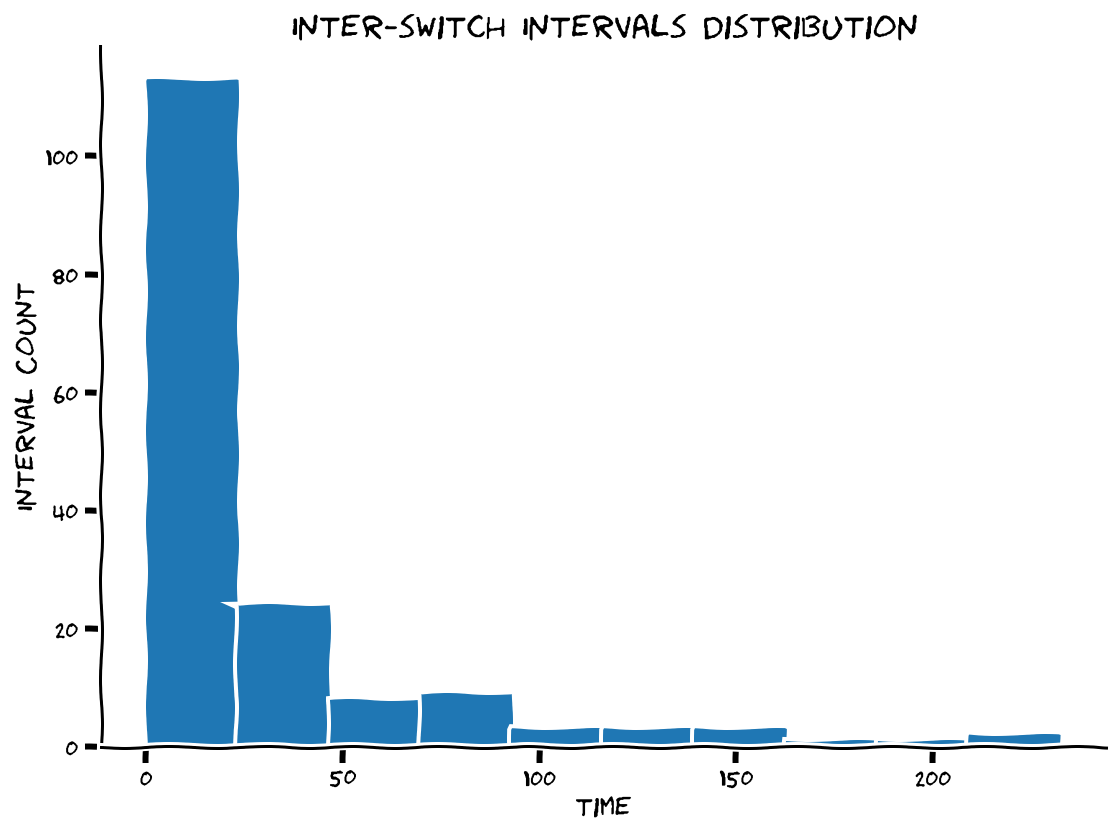
\includegraphics[scale=0.2]{Figures/LS/MC_Figure2.png}
\end{center}

We generate a bar graph to visualize the distribution of the number of time-steps spent in each of the two possible system states during the simulation.
\begin{center}
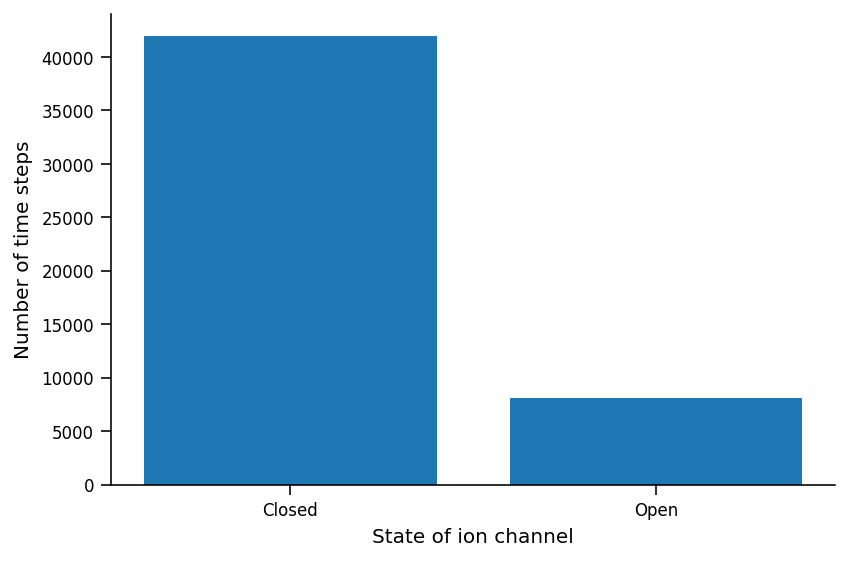
\includegraphics[scale=0.25]{Figures/LS/MC_Figure3.png}
\end{center}

Even though the state is discrete --the ion channel can only be either Closed or Open--we can still look at the \textit{mean state} of the system, averaged over some window of time. 

Since we've coded Closed as $x=0$ and Open as $x=1$, conveniently, the mean of $x$ over some window of time has the interpretation of \textit{fraction of time channel is Open}.

Let's also take a look at the fraction of Open states as a cumulative mean of the state $x$. The cumulative mean tells us the average number of state-changes that the system will have undergone after a certain amount of time. 

\begin{center}
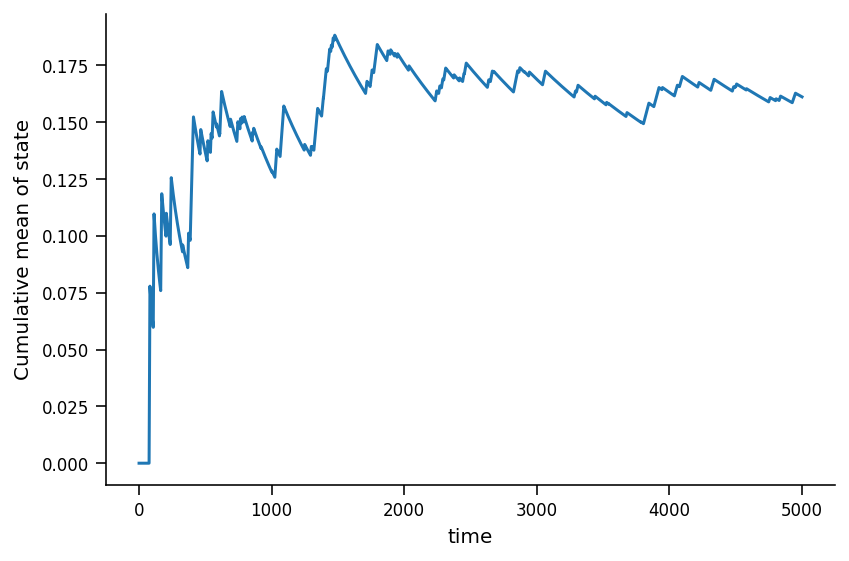
\includegraphics[scale=0.32]{Figures/LS/MC_Figure4.png}
\end{center}
\end{subbox}
\end{textbox}
%%%%%%%%%%%%%%%%%%%%%%%%% 
%%%%%%%%%%%%%%%%%%%%%%%%%
\begin{textbox}{\href{https://colab.research.google.com/github/NeuromatchAcademy/course-content/blob/master/tutorials/W2D2_LinearSystems/student/W2D2_Tutorial2.ipynb}{Markov Processes } }
\begin{subbox}{subbox}{Distributional Perspective}
\scriptsize
We can run a simulation many times and gather empirical distributions of open/closed states. Alternatively, we can formulate the exact same system probabilistically, keeping track of the probability of being in each state.

The same system of transitions can then be formulated using a vector of 2 elements as the state vector and a dynamics matrix $\mathbf{A}$. The result of this formulation is a *state transition matrix*:

\[\left[ \begin{array}{c} C \\ O \end{array} \right]_{k+1} = \mathbf{A} \left[ \begin{array}{c} C \\ O \end{array} \right]_k = \left[ \begin{matrix} 1-\mu_{\text{c2o}} & \mu_{\text{o2c}} \\ \mu_{\text{c2o}} & 1-\mu_{\text{o2c}} \end{matrix} \right] \left[ \begin{array}{c} C \\ O \end{array} \right]_k.\]


Each transition probability shown in the matrix is as follows:
\begin{enumerate}
    \item 
 $1-\mu_{\text{c2o}}$, the probability that the closed state remains closed. 
\item $\mu_{\text{c2o}}$, the probability that the closed state transitions to the open state.
\item  $\mu_{\text{o2c}}$, the probability that the open state transitions to the closed state. 
\item $1-\mu_{\text{o2c}}$, the probability that the open state remains open. 
\end{enumerate}



\textbf{Notice} that this system is written as a discrete step in time, and $\mathbf{A}$ describes the transition, mapping the state from step $k$ to step $k+1$. This is different from what we did in the exercises above where $\mathbf{A}$ had described the function from the state to the time derivative of the state.

\begin{center}
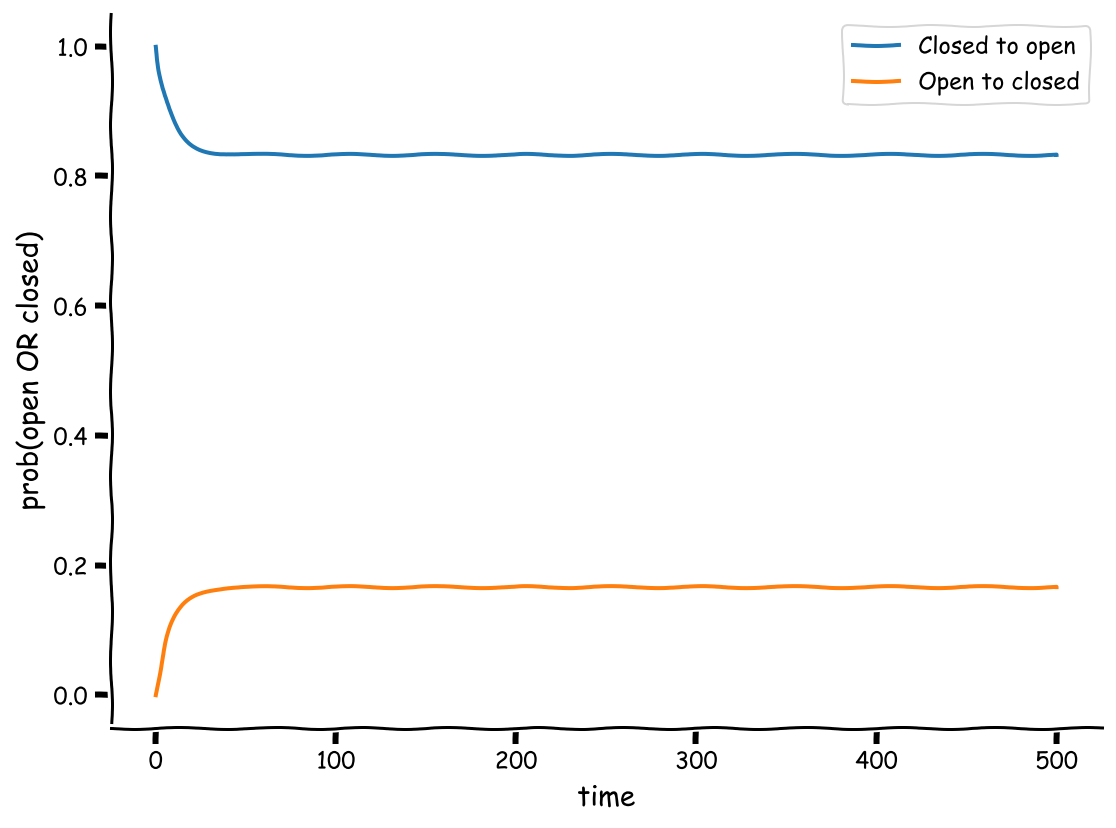
\includegraphics[scale=0.1]{Figures/LS/MC_Figure5.png}
\end{center}

\end{subbox}
\begin{subbox}{subbox}{Equilibrium of the telegraph process}
\scriptsize
Since we have now modeled the propagation of probabilities by the transition matrix $\mathbf{A}$ in Section 2, let's connect the behavior of the system at equilibrium with the eigendecomposition of $\mathbf{A}$.
The eigenvalues of $\mathbf{A}$ tell us about the stability of the system, specifically in the directions of the corresponding eigenvectors.

\end{subbox}
\end{textbox}
%%%%%%%%%%%%%%%%%%%%%%%%% 
%%%%%%%%%%%%%%%%%%%%%%%%%
% Combining determinism and stochasticity
%%%%%%%%%%%%%%%%%%%%%%%%% 
%%%%%%%%%%%%%%%%%%%%%%%%%
\begin{textbox}{\href{https://compneuro.neuromatch.io/tutorials/W2D2_LinearSystems/student/W2D2_Tutorial3.html}{Combining Determinism and Stochasticity } }
\begin{subbox}{subbox}{Introduction}
\scriptsize
We've spent some time familiarizing ourselves with the behavior of such systems when their trajectories are (1) entirely predictable and deterministic, or (2) governed by random processes, it's time to consider that neither is sufficient to describe neuroscience. Instead, we are often faced with processes for which we know some dynamics, but there are some random aspects as well. We call these \textbf{dynamical systems with stochasticity}.

\end{subbox}
\begin{subbox}{subbox}{Random Walks}
\scriptsize
To begin, let's first take a gander at how life sometimes wanders around aimlessly. One of the simplest and best-studied living systems that has some interesting behaviors is the \textit{E. coli} bacterium, which is capable of navigating odor gradients on a substrate to seek a food source. Larger life (including flies, dogs, and blindfolded humans) sometimes use the same strategies to guide their decisions.

Here, we will consider what the \textit{E. coli} does in the absence of food odors. What's the best strategy when one does not know where to head? Why, flail around randomly, of course!

The \textbf{random walk} is exactly that --- at every time step, use a random process like flipping a coin to change one's heading accordingly. Note that this process is closely related to \textbf{Brownian motion}, so you may sometimes hear that terminology used as well.

Let's start with a \textbf{one-dimensional random walk}. A bacterium starts at $x=0$. At every time step, it flips a coin (a very small, microscopic coin of protein mintage), then heads left $\Delta x = -1$ or right $\Delta x = +1$ for with equal probability. For instance, if at time step $1$ the result of the coin flip is to head right, then its position at that time step becomes $x_1 = x_0 + \Delta x = 1.$ Continuing in this way, its position at time step $k+1$ is given by 
$$x_{k+1} = x_k + \Delta x $$    

We will simulate this process below and plot the position of the bacterium as a function of the time step.
\begin{center}
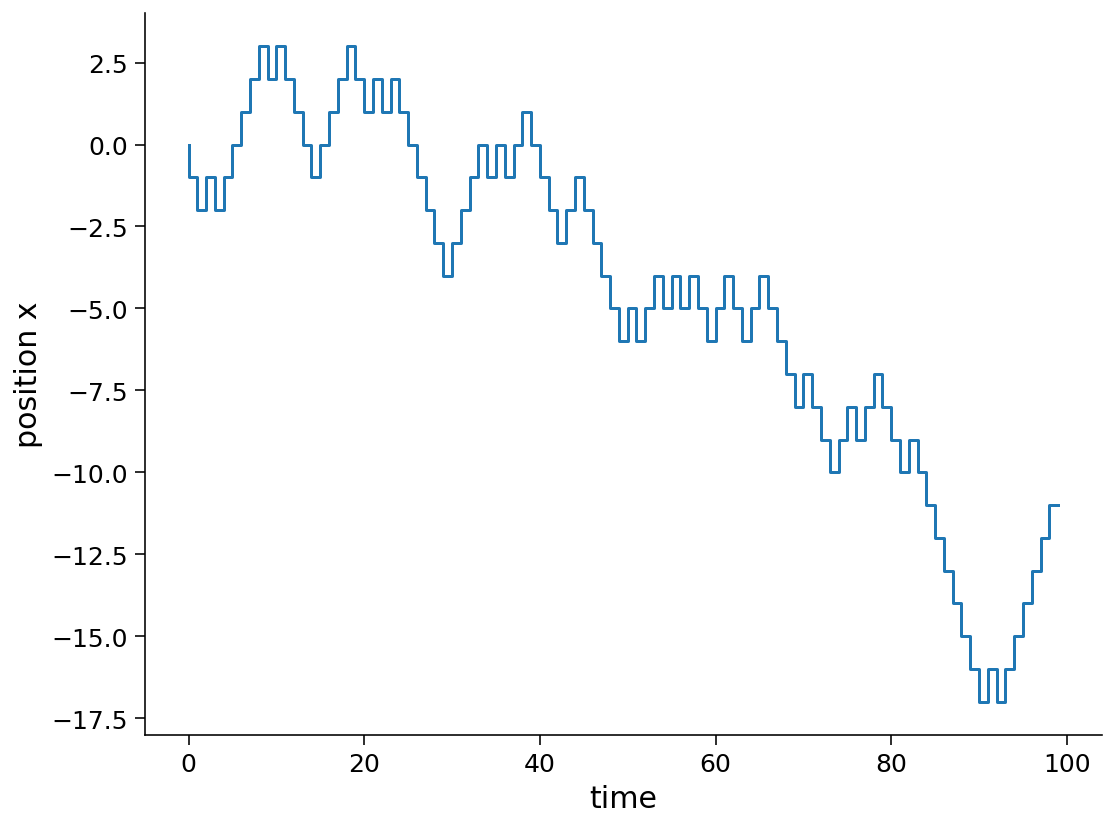
\includegraphics[scale=0.25]{Figures/LS/CDS_Figure1.png}
\end{center}
\end{subbox}
\end{textbox}
%%%%%%%%%%%%%%%%%%%%%%%%% 
%%%%%%%%%%%%%%%%%%%%%%%%%
\begin{textbox}{\href{https://compneuro.neuromatch.io/tutorials/W2D2_LinearSystems/student/W2D2_Tutorial3.html}{Combining Determinism and Stochasticity } }

\begin{subbox}{subbox}{Random Walks Simulations}
\scriptsize
We will plot 10 random walks for 10000 time steps each where the steps have a standard normal distribution (with mean $\mu$ and standard deviation $\sigma$). 


\begin{center}
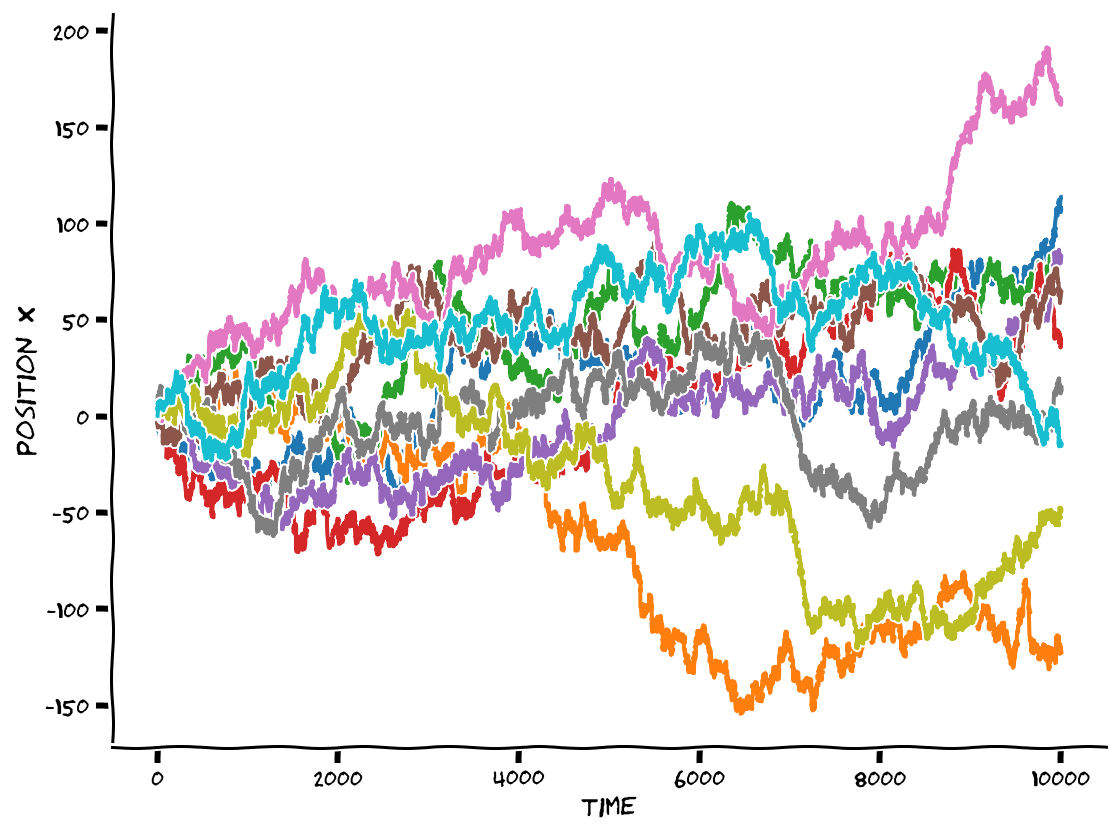
\includegraphics[scale=0.25]{Figures/LS/CDS_Figure3.png}
\end{center}

We see that the trajectories all look a little different from each other. But there are some general observations one can make: at the beginning almost all trajectories are very close to $x=0$, which is where our bacterium started. As time progresses, some trajectories move further and further away from the starting point. However, a lot of trajectories stay close to the starting point of $x=0$. 

Now let's take a look in the next cell at the distribution of bacteria positions at different points in time, analyzing all the trajectories from above.
\begin{center}
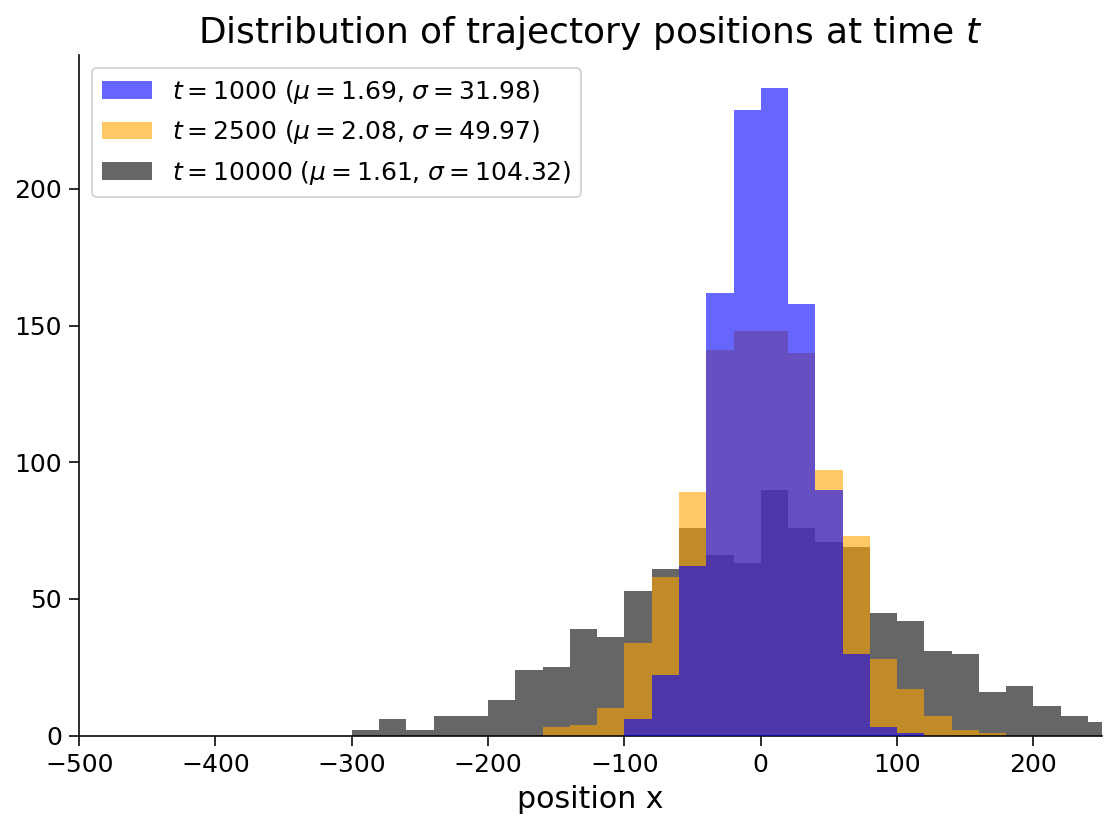
\includegraphics[scale=0.25]{Figures/LS/CDS_Figure4.png}
\end{center}
The plot of the mean and variance of our bacterium's random walk as a function of time.

\begin{center}
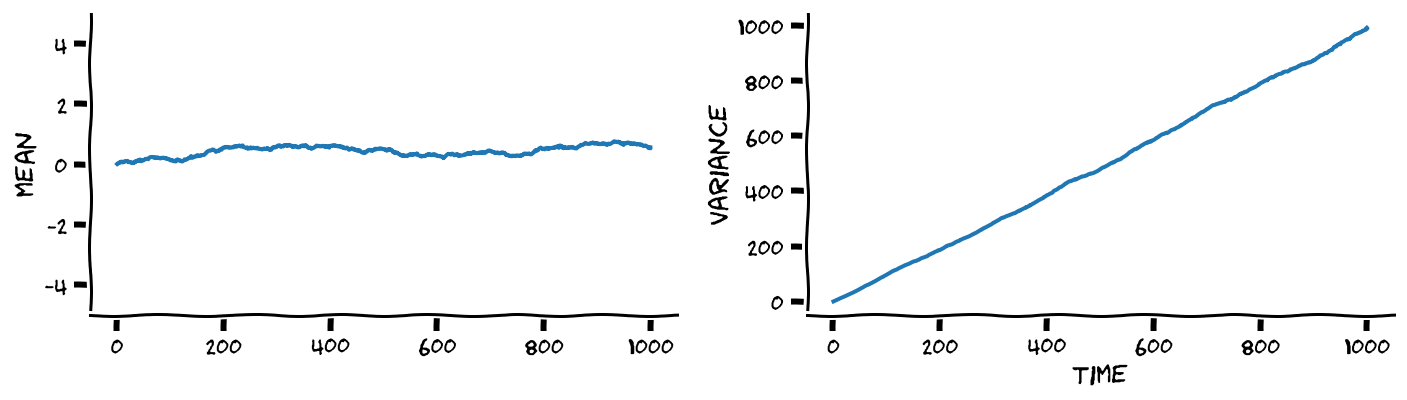
\includegraphics[scale=0.25]{Figures/LS/CDS_Figure5.png}
\end{center}
\end{subbox}
\end{textbox}

%%%%%%%%%%%%%%%%%%%%%%%%% 
%%%%%%%%%%%%%%%%%%%%%%%%%
\begin{textbox}{\href{https://compneuro.neuromatch.io/tutorials/W2D2_LinearSystems/student/W2D2_Tutorial3.html}{Combining Determinism and Stochasticity } }

\begin{subbox}{subbox}{The Ornstein-Uhlenbeck (OU) process}
\scriptsize
Our goal is now to build on this model to construct a \textbf{drift-diffusion} model (DDM). DDM is a popular model for memory, which as we all know, is often an exercise in hanging on to a value imperfectly. Decision-making and memory will be the topic for tomorrow, so here we build the mathematical foundations and develop some intuition for how such systems behave!

To build such a model, let's combine the random walk model with the first order discrete differential equation. We have to modify our analytic solution of the differential equation slightly:

\[x_k = x_\infty(1 - \lambda^k) + x_0 \lambda^k.\]

The dynamics of this process starts at $x_0$ and decay towards $x_{\infty}.$

Now we are ready to take this basic, deterministic difference equation and add a diffusion process on top of it!

As a point of terminology: this type of process is commonly known as a \textbf{drift-diffusion model} or \textbf{Ornstein-Uhlenbeck (OU) process}. The model is a combination of a drift term toward $x_{\infty}$ and a diffusion term that walks randomly. You may sometimes see them written as continuous stochastic differential equations, but here we are doing the discrete version to maintain continuity in the tutorial. The discrete version of our OU process has the following form:

\[x_{k+1} = x_\infty + \lambda(x_k - x_{\infty}) + \sigma \eta\]

where $\eta$ is sampled from a standard normal distribution ($\mu=0, \sigma=1$). 
\begin{center}
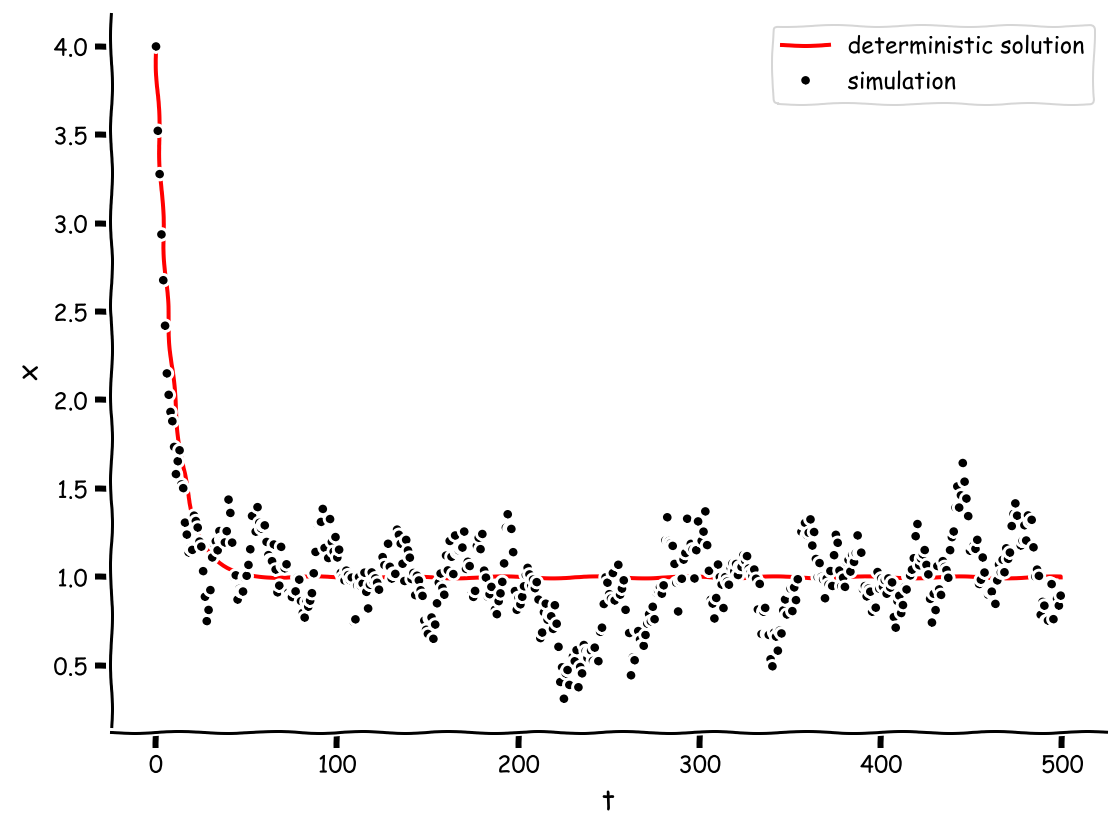
\includegraphics[scale=0.08]{Figures/LS/CDS_Figure7.png}
\end{center}
\end{subbox}
\begin{subbox}{subbox}{Variance of the OU process}
\scriptsize

As we can see, the \textit{mean} of the process follows the solution to the deterministic part of the governing equation. But what about the \texit{variance}? 

Unlike the random walk, because there's a decay process that "pulls" $x$ back towards $x_\infty$, the variance does not grow without bound with large $t$. Instead, when it gets far from $x_\infty$, the position of $x$ is restored, until an equilibrium is reached.

The equilibrium variance for our drift-diffusion system is

\[\text{Var} = \frac{\sigma^2}{1 - \lambda^2}.\]

Notice that the value of this equilibrium variance depends on $\lambda$ and $\sigma$. It does not depend on $x_0$ and $x_\infty$.

\end{subbox}

\end{textbox}

%%%%%%%%%%%%%%%%%%%%%%%%% 
%%%%%%%%%%%%%%%%%%%%%%%%%
%%% Autoregressive models
%%%%%%%%%%%%%%%%%%%%%%%%% 
%%%%%%%%%%%%%%%%%%%%%%%%%
\begin{textbox}{\href{https://compneuro.neuromatch.io/tutorials/W2D2_LinearSystems/student/W2D2_Tutorial4.html}{Autoregressive models } }
\begin{subbox}{subbox}{Fitting data to the OU process}
\scriptsize
 Our process  the drift-diffusion (OU) process had following form:
\[x_{k+1} = x_{\infty} + \lambda(x_k - x_{\infty}) + \sigma \eta\]
where $\eta$ is sampled from a standard normal distribution. 
For simplicity, we set $x_\infty = 0$. Let's plot a trajectory for this process again below. Take note of the parameters of the process because they will be important later.

\begin{center}
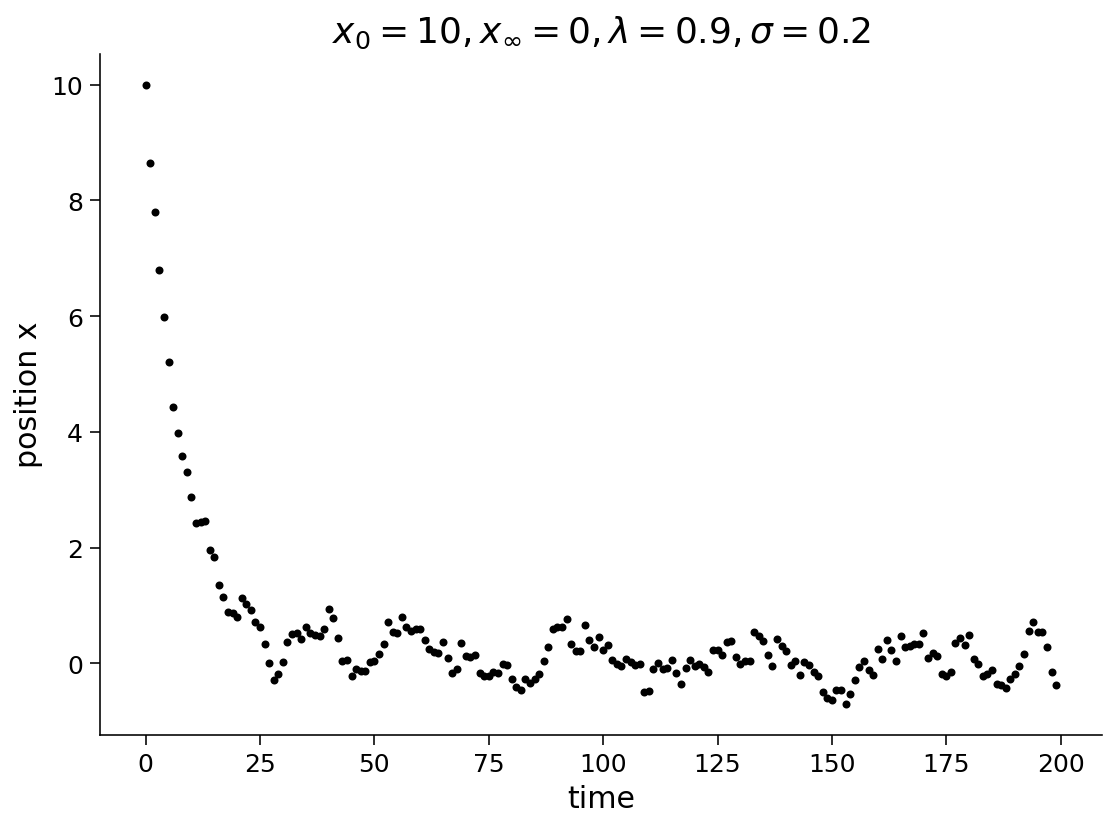
\includegraphics[scale=0.25]{Figures/LS/CDS_Figure8.png}
\end{center}
What if we were given these positions $x$ as they evolve in time as data, how would we get back out the dynamics of the system $\lambda$? 

Since a little bird told us that this system takes on the form

$$x_{k+1} = \lambda x_k + \eta,$$

where $\eta$ is noise from a normal distribution, our approach is to solve for $\lambda$ as a \textbf{regression problem}. 

As a check, let's plot every pair of points adjacent in time ($x_{k+1}$ vs. $x_k$) against each other to see if there is a linear relationship between them. 

Hooray, it's a line! This is evidence that the dynamics that generated the data is linear. We can now reformulate this task as a regression problem.
\begin{center}
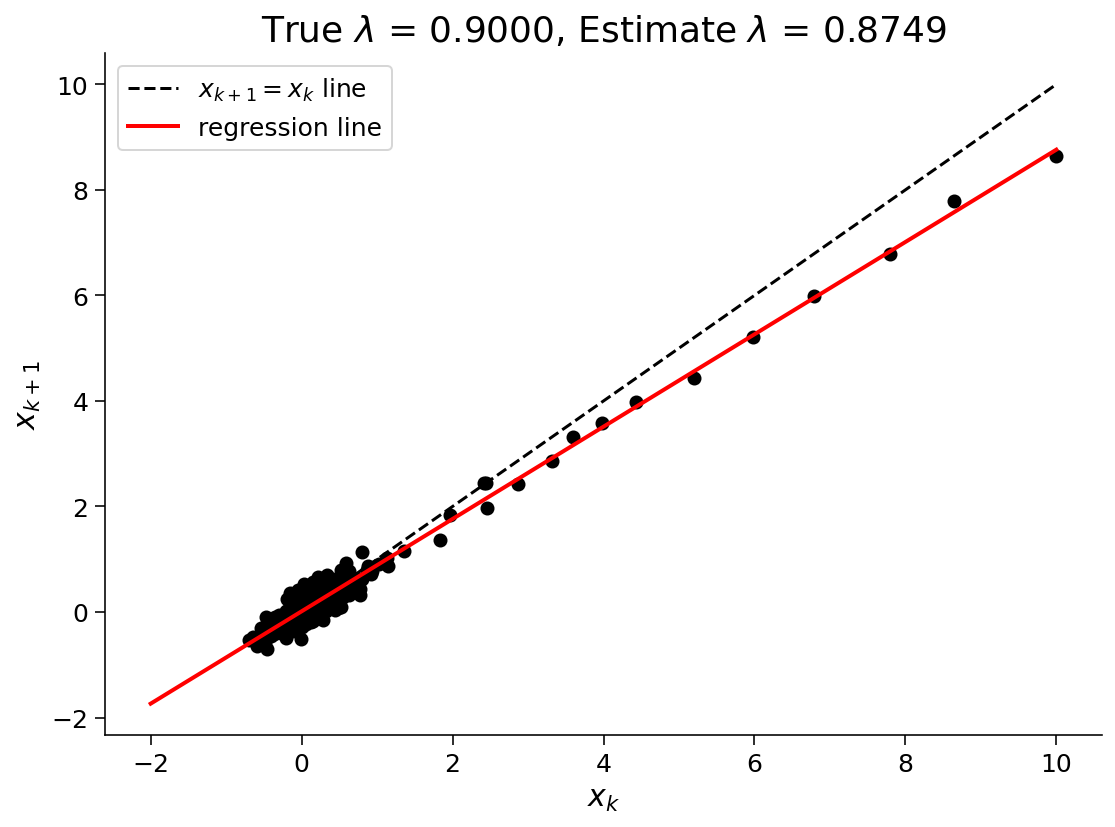
\includegraphics[scale=0.25]{Figures/LS/CDS_Figure10.png}
\end{center}
This model is \textbf{autoregressive}, where auto means self. In other words, it's a regression of the time series on itself from the past. The equation as written above is only a function of itself from one step in the past, so we can call it a first order autoregressive model and plot.


\end{subbox}

\end{textbox}
%%%%%%%%%%%%%%%%%%%%%%%%% 
%%%%%%%%%%%%%%%%%%%%%%%%%
\begin{textbox}{\href{https://compneuro.neuromatch.io/tutorials/W2D2_LinearSystems/student/W2D2_Tutorial4.html}{Autoregressive models } }
\begin{subbox}{subbox}{Higher order autoregressive models}
\scriptsize
Now that we have established the autoregressive framework, generalizing for dependence on data points from the past is straightforward. \textbf{Higher order} autoregression models a future time point based on more than one point in the past.

In one dimension, we can write such an order-$r$ model as
$$
x_{k+1} = \alpha_0 + \alpha_1 x_k + \alpha_2 x_{k-1} + \alpha_3 x_{k-2} + \dots + \alpha_{r+1} x_{k-r} \text{  , }
$$
where the $\alpha$'s are the $r+1$ coefficients to be fit to the data available.

These models are useful to account for some \textbf{history dependence} in the trajectory of time series. This next part of the tutorial will explore one such time series, and you can do an experiment on yourself!

In particular, we will explore a binary random sequence of 0's and 1's that would occur if you flipped a coin and jotted down the flips. 

The difference is that, instead of actually flipping a coin (or using code to generate such a sequence), you -- yes you, human -- are going to generate such a random Bernoulli sequence as best as you can by typing in 0's and 1's. We will then build higher-order AR models to see if we can identify predictable patterns in the time-history of digits you generate.
\begin{center}
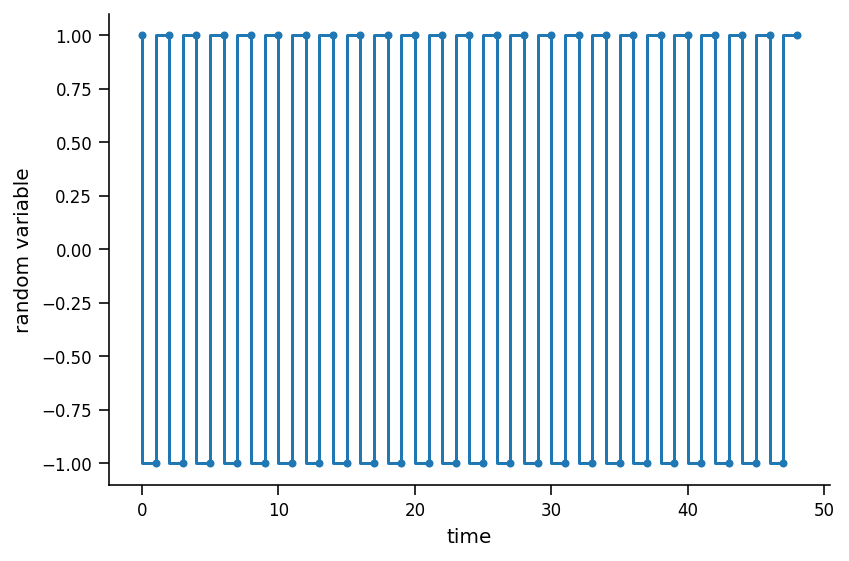
\includegraphics[scale=0.4]{Figures/LS/CDS_Figure11.png}
\end{center}

\end{subbox}

\end{textbox}

%%%%%%%%%%%%%%%%%%%%%%%%% 
%%%%%%%%%%%%%%%%%%%%%%%%%
\begin{textbox}{\href{https://compneuro.neuromatch.io/tutorials/W2D2_LinearSystems/student/W2D2_Tutorial4.html}{Autoregressive models } }

\begin{subbox}{subbox}{Understanding autoregressive parameters}
\scriptsize
Truly random sequences of numbers have no structure and should not be predictable by an AR or any other models.

However, humans are notoriously terrible at generating random sequences of numbers! (Other animals are no better...)

To test out an application of higher-order AR models, let's use them to model a sequence of 0's and 1's that a human tried to produce at random. 

If the digits really have no structure, then we expect our model to do about as well as guessing, producing an error rate of 0.5. Let's see how well we can do!

Fit a order-5 ($r=5$) AR model to the data vector $x$. We will then plot the observations against the trained model. Note that this means we are using a sequence of the previous 5 digits to predict the next one. 

Additionally, output from our regression model is continuous (real numbers) whereas our data are scalar (+1/-1). So, we will take the sign of our continuous outputs (+1 if positive and -1 if negative) as our predictions to make them comparable with data. Our error rate will simply be the number of mismatched predictions divided by the total number of predictions.
\begin{center}
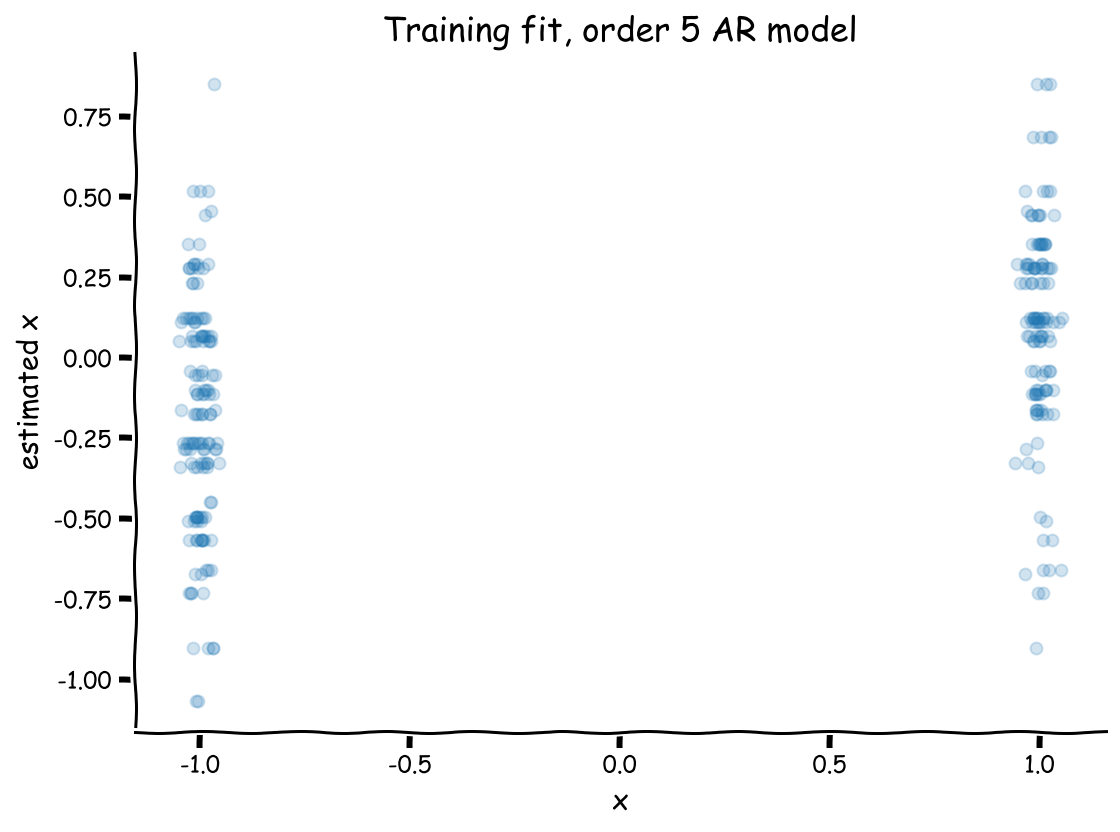
\includegraphics[scale=0.15]{Figures/LS/CDS_Figure12.png}
\end{center}
Let's now try \textbf{AR models of different orders} systematically, and plot the test error of each.

\begin{center}
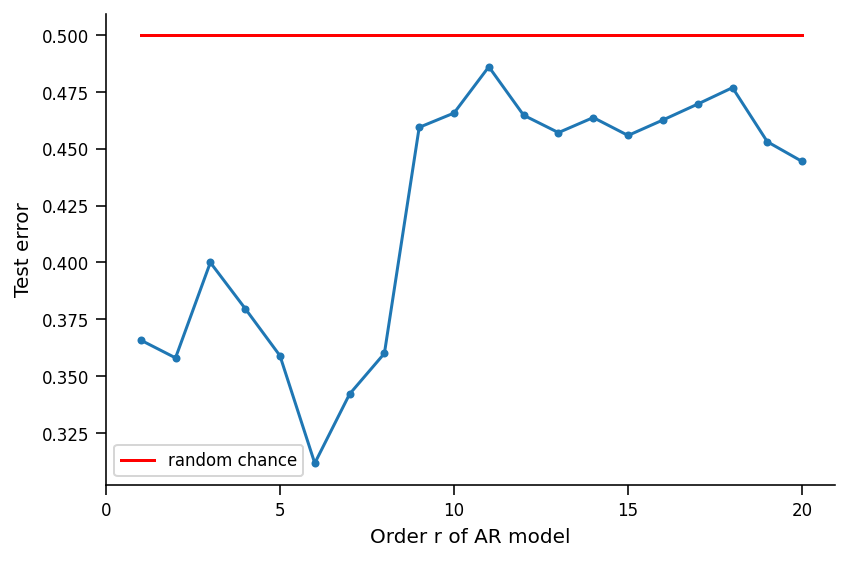
\includegraphics[scale=0.35]{Figures/LS/CDS_Figure13.png}
\end{center}


Notice that there's a sweet spot in the test error! The 6th order AR model does a really good job here, and for larger $r$'s, the model starts to overfit the training data and does not do well on the test data.

\end{subbox}
\end{textbox}
\end{multicols}



\includegraphics[scale=0.03]{Figures/NMACN.png}\href{https://compneuro.neuromatch.io/tutorials/intro.html}{\textbf{\Huge{Neuromatch Academy: Biological Neuron Models - Summary Sheet}}\footnote{’t Hart et al., (2022). Neuromatch Academy: a 3-week, online summer school in computational neuroscience. Journal of Open Source Education, 5(49), 118. https://doi.org/10.21105/jose.00118}}
\begin{multicols}{3}
\clearpage
\begin{textbox}{\href{https://compneuro.neuromatch.io/tutorials/W1D4_GeneralizedLinearModels/student/W1D4_Tutorial1.html}{Generalized Linear Models (W1D4T1)} }
\begin{subbox}{subbox}{Create design matrix}
\scriptsize

To create the \textbf{design matrix} which organizes the stimulus intensities in matrix form such that the $i$th row has the stimulus frames preceding timepoint $i$.

In this example, we will create the design matrix $\mathbf{X}$ using $d=25$ time lags. That is, $\mathbf{X}$ should be a $T \times d$ matrix. $d = 25$  is a choice we're making based on our prior knowledge of the temporal window that influences RGC responses. 

\centering
\includegraphics[scale=0.15]{Figures/GLM/GLMFigure1.png}
\end{subbox}

\begin{subbox}{subbox}{Fit Linear-Gaussian regression model 
}
\scriptsize{The maximum likelihood estimate of $\theta$ in this model can be solved analytically using the equation:

\begin{align}
\boldsymbol{\hat \theta} = (\mathbf{X}^{\top}\mathbf{X})^{-1}\mathbf{X}^{\top}\mathbf{y}.
\end{align}}
The resulting maximum likelihood filter estimates are:
\centering
\includegraphics[scale=0.22]{Figures/GLM/GLMFigure2.png}
\end{subbox}
\end{textbox}
%%%%%%%%%%%%%%%%%%%%%%%%%%%%%%%%%%%%%%%%%%%%%%%%%%
%%%%%%%%%%%%%%%%%%%%%%%%%%%%%%%%%%%%%%%%%%%%%%%%%%
\begin{textbox}{\href{https://compneuro.neuromatch.io/tutorials/W1D4_GeneralizedLinearModels/student/W1D4_Tutorial1.html}{Generalized Linear Models (W1D4T1)} }
\begin{subbox}{subbox}{Create design matrix}
\scriptsize
Poisson regression is a generalized linear model form of regression analysis used to model count data, like spikes.
In the Poisson GLM,
\begin{align}
\log P(\mathbf{y} \mid \mathbf{X}, \theta) = \sum_t \log P(y_t \mid \mathbf{x_t},\theta),
\end{align}
where
\begin{align}
P(y_t \mid \mathbf{x_t}, \theta) = \frac{\lambda_t^{y_t}\exp(-\lambda_t)}{y_t!} \text{, with rate } \lambda_t = \exp(\mathbf{x_t}^{\top} \theta).
\end{align}

Now, taking the log likelihood for all the data we obtain:
$\log P(\mathbf{y} \mid X, \theta) = \sum_t( y_t \log\left(\lambda_t) - \lambda_t - \log(y_t !)\right).$

Because we are going to minimize the negative log likelihood with respect to the parameters $\theta$, we can ignore the last term that does not depend on $\theta$. For faster implementation, let us rewrite this in matrix notation:

\begin{align}
\mathbf{y}^{\top} \log(\mathbf{\lambda}) - \mathbf{1}^{\top} \mathbf{\lambda} \text{, with  rate } \mathbf{\lambda} = \exp(\mathbf{X} \theta)
\end{align}

Finally, don't forget to add the minus sign for your function to return the negative log likelihood.

\centering
\includegraphics[scale=0.11]{Figures/GLM/GLMFigure3.png}
\end{subbox}

\begin{subbox}{subbox}{Spike Prediction 
}

\centering
\includegraphics[scale=0.11]{Figures/GLM/GLMFigure4.png}
\end{subbox}
\end{textbox}
\begin{textbox}{\href{https://compneuro.neuromatch.io/tutorials/W1D4_GeneralizedLinearModels/student/W1D4_Tutorial2.html}{Generalized Linear Models (W1D4T2)} }
\begin{subbox}{subbox}{Logistic regression}
\scriptsize
Logistic Regression is a binary classification model. It is a GLM with a logistic link function and a Bernoulli (i.e. coinflip) noise model.
The fundamental input/output equation of logistic regression is:

\begin{align}
\hat{y} \equiv p(y=1|x,\theta) = \sigma(\theta^Tx)
\end{align}

Note that we interpret the output of logistic regression, $\hat{y}$, as the probability that $y = 1$ given inputs $x$ and parameters $\theta$.

Here $\sigma()$ is a "squashing" function called the sigmoid function or logistic function. Its output is in the range $0 \leq y \leq 1$. It looks like this:

\begin{align}
\sigma(z) = \frac{1}{1 + \textrm{exp}(-z)}
\end{align}
Recall that $z = \theta^T x$. The parameters decide whether $\theta^T x$ will be very negative, in which case $\sigma(\theta^T x)\approx 0$, or very positive, meaning  $\sigma(\theta^T x)\approx 1$.

\centering
\includegraphics[scale=0.08]{Figures/GLM/GLMFigure5.png}
\end{subbox}

\begin{subbox}{subbox}{Regularisation 
}
\scriptsize
Regularization forces a model to learn a set solutions you a priori believe to be more correct, which reduces over-fitting because it doesn't have as much flexibility to fit idiosyncrasies in the training data. This adds model bias, but it's a good bias because you know (maybe) that parameters should be small or mostly 0.

\textbf{$L_2$ regularization}
Regularization comes in different flavors. A very common one uses an $L_2$ or "ridge" penalty. This changes the objective function to

\begin{align}
-\log\mathcal{L}'(\theta | X, y)=
-\log\mathcal{L}(\theta | X, y) +\frac\beta2\sum_i\theta_i^2,
\end{align}
where $\beta$ is a *hyperparameter* that sets the *strength* of the regularization.
\end{subbox}
\end{textbox}
%%%%%%%%%%%%%%%%%%%%%%%%%%%%%%%%%%%%%%%%%%%%%%%%%%%%%%
%%%%%%%%%%%%%%%%%%%%%%%%%%%%%%%%%%%%%%%%%%%%%%%%%%%%%%

\end{multicols}
\newpage

\includegraphics[scale=0.03]{Figures/NMACN.png}\href{https://compneuro.neuromatch.io/tutorials/intro.html}{\textbf{\Huge{Neuromatch Academy: Dynamic Networks - Summary Sheet}}\footnote{’t Hart et al., (2022). Neuromatch Academy: a 3-week, online summer school in computational neuroscience. Journal of Open Source Education, 5(49), 118. https://doi.org/10.21105/jose.00118}}
\begin{multicols}{3}

\begin{textbox}{\href{https://compneuro.neuromatch.io/tutorials/W2D4_DynamicNetworks/chapter_title.html}{Neural Rate Models (W2D4T1)} }
\begin{subbox}{subbox}{Dynamics of a single excitatory population}
\scriptsize
Individual neurons respond by spiking. When we average the spikes of neurons in a population, we can define the average firing activity of the population. In this model, we are interested in how the population-averaged firing varies as a function of time and network parameters. Mathematically, we can describe the firing rate dynamic of a feed-forward network as:
$$ \tau \frac{dr}{dt} &= -r + F(I_{\text{ext}})  \quad $$
$r(t)$ represents the average firing rate of the excitatory population at time $t$, $\tau$ controls the timescale of the evolution of the average firing rate, $I_{\text{ext}}$ represents the external input, and the transfer function $F(\cdot)$ (which can be related to f-I curve of individual neurons described in the next sections) represents the population activation function in response to all received inputs.


\end{subbox}
\begin{subbox}{subbox}{F-I (firing rate vs. input) curve}
\scriptsize
In electrophysiology, a neuron is often characterized by its spike rate output in response to input currents. This is often called the F-I curve, denoting the output spike frequency (F) in response to different injected currents (I). 

The transfer function $F(\cdot)$ in Equation $1$ represents the gain of the population as a function of the total input. The gain is often modeled as a sigmoidal function, i.e., more input drive leads to a nonlinear increase in the population firing rate. The output firing rate will eventually saturate for high input values. 

A sigmoidal $F(\cdot)$ is parameterized by its gain $a$ and threshold $\theta$.
$$ F(x;a,\theta) = \frac{1}{1+\text{e}^{-a(x-\theta)}} - \frac{1}{1+\text{e}^{a\theta}} $$

The argument $x$ represents the input to the population. Note that the second term is chosen so that $F(0;a,\theta)=0$.

\begin{center}
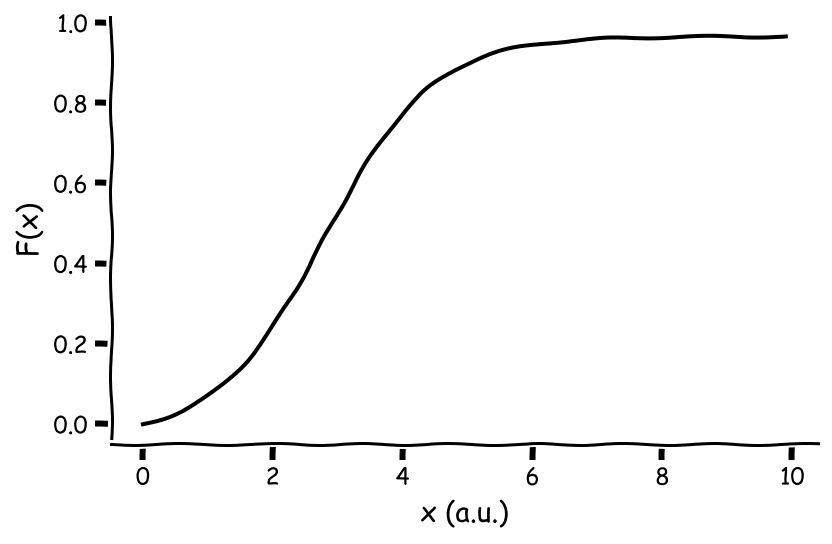
\includegraphics[scale=0.18]{Figures/DN/DN_Figure1.png}
\end{center}
\end{subbox}

\end{textbox}
%%%%%%%%%%%%%%%%%%%%%%%%%%%%%%%%%%%%%%%%%%%%%%%%%%%%%%
%%%%%%%%%%%%%%%%%%%%%%%%%%%%%%%%%%%%%%%%%%%%%%%%%%%%%%
\begin{textbox}{\href{https://compneuro.neuromatch.io/tutorials/W2D4_DynamicNetworks/chapter_title.html}{Neural Rate Models (W2D4T1)} }
\begin{subbox}{subbox}{Fixed points of the single population system}
\scriptsize
We can now extend our feed-forward network to a recurrent network, governed by the equation:

\begin{equation*}
\tau \frac{dr}{dt} &= -r + F(w\cdot r + I_{\text{ext}})  \quad\qquad (+)
\end{equation*}

where as before, $r(t)$ represents the average firing rate of the excitatory population at time $t$, $\tau$ controls the timescale of the evolution of the average firing rate, $I_{\text{ext}}$ represents the external input, and the transfer function $F(\cdot)$ (which can be related to f-I curve of individual neurons described in the next sections) represents the population activation function in response to all received inputs. Now we also have $w$ which denotes the strength (synaptic weight) of the recurrent input to the population.

As you varied the two parameters in the last Interactive Demo, you noticed that, while at first the system output quickly changes, with time, it reaches its maximum/minimum value and does not change anymore. The value eventually reached by the system is called the \textbf{steady state} of the system, or the \textbf{fixed point}. Essentially, in the steady states the derivative with respect to time of the activity ($r$) is zero, i.e. $\displaystyle \frac{dr}{dt}=0$. 

We can find that the steady state of the Equation ($+$) by setting $\displaystyle{\frac{dr}{dt}=0}$ and solve for $r$:
\begin{equation*}
-r_{\text{steady}} + F(w\cdot r_{\text{steady}} + I_{\text{ext}};a,\theta) = 0 \qquad (\ddagger)
\end{equation*}
When it exists, the solution of Equation ($\ddagger$) defines a \textbf{fixed point} of the dynamical system in Equation ($+$). Note that if $F(x)$ is nonlinear, it is not always possible to find an analytical solution, but the solution can be found via numerical simulations.
In the specific case of $w=0$, we can also analytically compute  the solution of Equation ($+$) and deduce the role of $\tau$ in determining the convergence to the fixed point: 
\begin{equation*}
\displaystyle{r(t) = \big{[}F(I_{\text{ext}};a,\theta) -r(t=0)\big{]} (1-\text{e}^{-\frac{t}{\tau}})} + r(t=0)
\end{equation*}
We can now numerically calculate the fixed point with a root finding algorithm.
\begin{center}
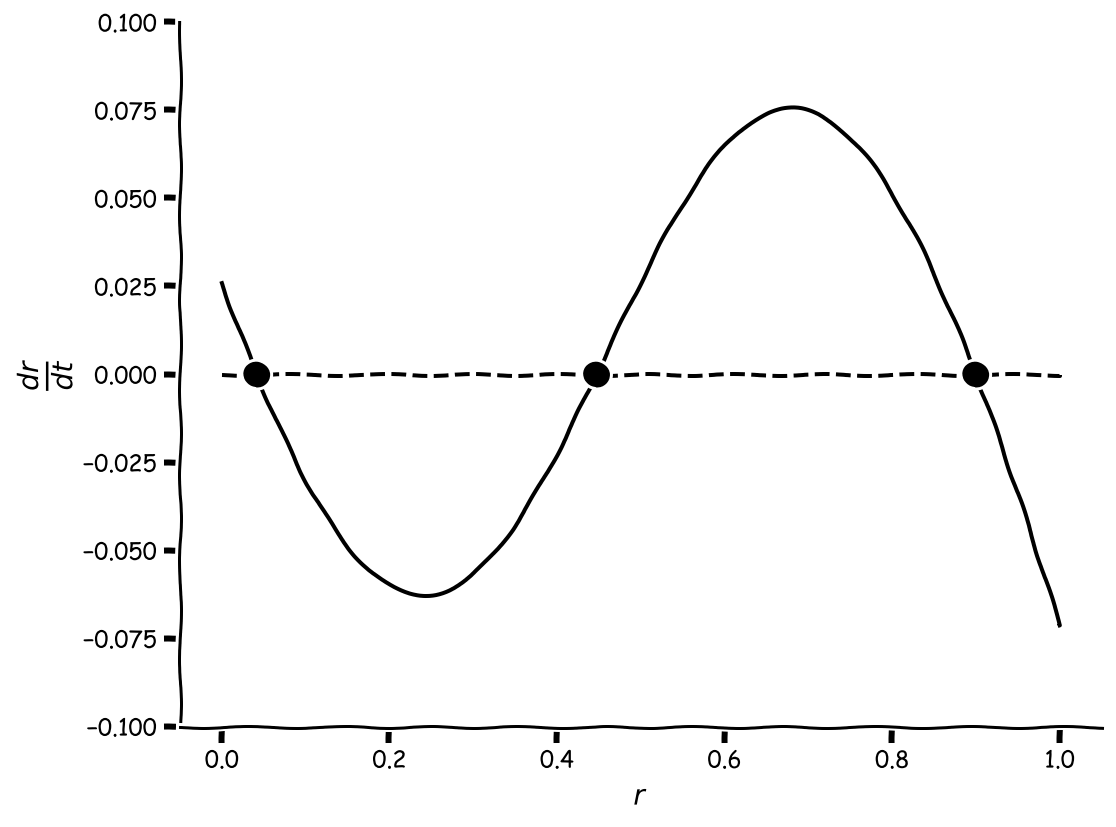
\includegraphics[scale=0.1]{Figures/DN/DN_Figure2.png}
\end{center}
\end{subbox}

\end{textbox}
%%%%%%%%%%%%%%%%%%%%%%%%%%%%%%%%%%%%%%%%%%%%%%%%%%%%%%
%%%%%%%%%%%%%%%%%%%%%%%%%%%%%%%%%%%%%%%%%%%%%%%%%%%%%%
\begin{textbox}{\href{https://compneuro.neuromatch.io/tutorials/W2D4_DynamicNetworks/chapter_title.html}{Neural Rate Models (W2D4T1)} }
\begin{subbox}{subbox}{Fixed points of the single population system}
\scriptsize
Relationship between trajectories & fixed points

Let's examine the relationship between the population activity over time and the fixed points.

Here, let us first set $w=5.0$ and $I_{\text{ext}}=0.5$, and investigate the dynamics of $r(t)$ starting with different initial values $r(0) \equiv r_{\text{init}}$. 


We will plot the trajectories of $r(t)$ with different initial values $r(0) \equiv r_{\text{init}}  = 0.0, 0.1, 0.2,..., 0.9$.
We have three fixed points but only two steady states showing up - what's happening? 

It turns out that the stability of the fixed points matters. If a fixed point is stable, a trajectory starting near that fixed point will stay close to that fixed point and converge to it (the steady state will equal the fixed point). If a fixed point is unstable, any trajectories starting close to it will diverge and go towards stable fixed points. In fact, the only way for a trajectory to reach a stable state at an unstable fixed point is if the initial value \textbf{exactly} equals the value of the fixed point.

We can simulate the trajectory if we start at the unstable fixed point: you can see that it remains at that fixed point (the red line below).

\begin{center}
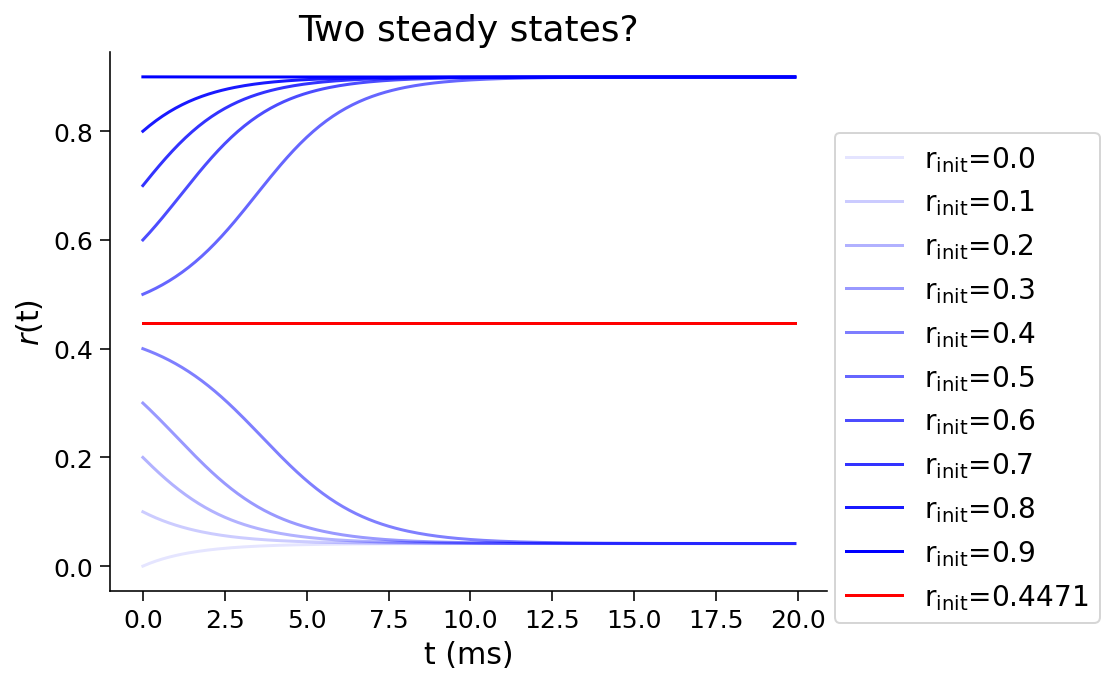
\includegraphics[scale=0.3]{Figures/DN/DN_Figure4.png}
\end{center}
\end{subbox}

\end{textbox}
%%%%%%%%%%%%%%%%%%%%%%%%%%%%%%%%%%%%%%%%%%%%%%%%%%%%%%
%%%%%%%%%%%%%%%%%%%%%%%%%%%%%%%%%%%%%%%%%%%%%%%%%%%%%%
\begin{textbox}{\href{https://compneuro.neuromatch.io/tutorials/W2D4_DynamicNetworks/chapter_title.html}{Wilson-Cowan Model (W2D4T2)} }
\begin{subbox}{subbox}{Mathematical description of the WC model}
\scriptsize
Many of the rich dynamics recorded in the brain are generated by the interaction of excitatory and inhibitory subtype neurons. Here, similar to what we did in the previous tutorial, we will model two coupled populations of E and I neurons (\textbf{Wilson-Cowan} model). We can write two coupled differential equations, each representing the dynamics of the excitatory or inhibitory population:

\begin{align*}
\tau_E \frac{dr_E}{dt} &= -r_E + F_E(w_{EE}r_E -w_{EI}r_I + I^{\text{ext}}_E;a_E,\theta_E)\\
\tau_I \frac{dr_I}{dt} &= -r_I + F_I(w_{IE}r_E -w_{II}r_I + I^{\text{ext}}_I;a_I,\theta_I)    
\end{align*}

$r_E(t)$ represents the average activation (or firing rate) of the excitatory population at time $t$, and $r_I(t)$ the activation (or firing rate) of the inhibitory population. The parameters $\tau_E$ and $\tau_I$ control the timescales of the dynamics of each population. Connection strengths are given by: $w_{EE}$ (E $\rightarrow$ E), $w_{EI}$ (I $\rightarrow$ E), $w_{IE}$ (E $\rightarrow$ I), and $w_{II}$ (I $\rightarrow$ I). The terms $w_{EI}$ and $w_{IE}$ represent connections from inhibitory to excitatory population and vice versa, respectively. The transfer functions (or F-I curves) $F_E(x;a_E,\theta_E)$ and $F_I(x;a_I,\theta_I)$ can be different for the excitatory and the inhibitory populations.
\begin{center}
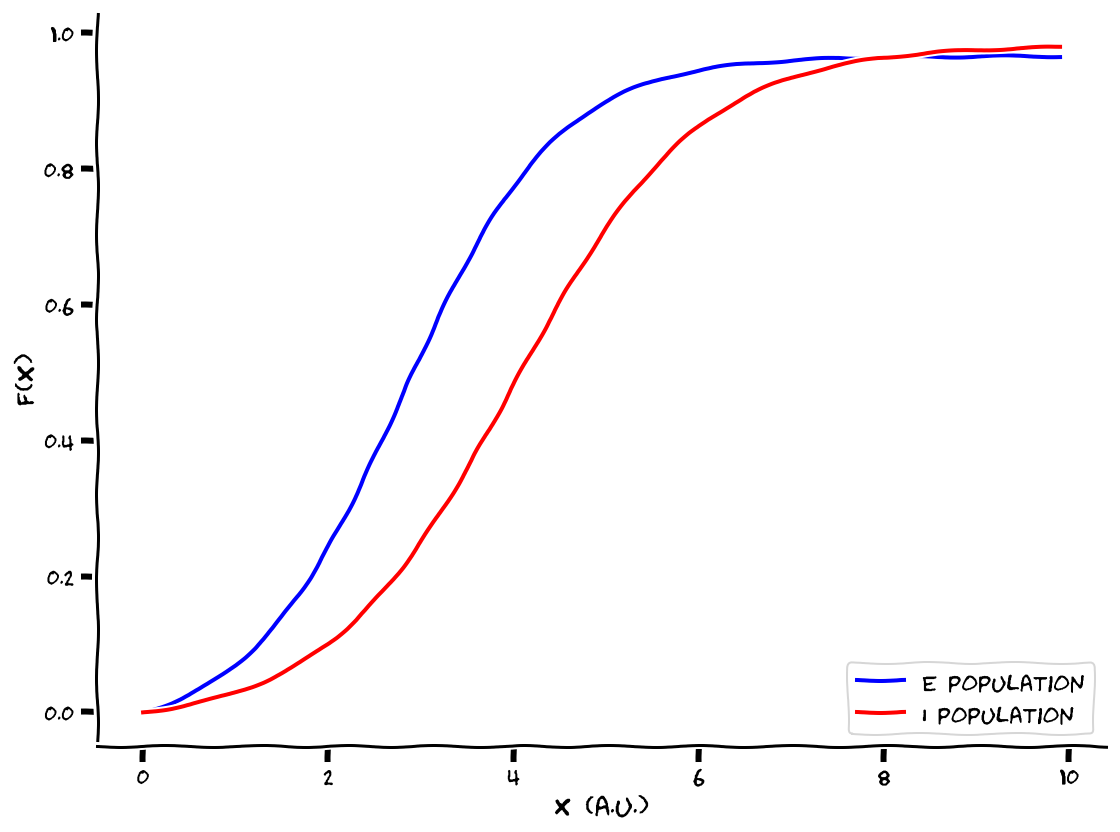
\includegraphics[scale=0.18]{Figures/DN/DN_Figure5.png}
\end{center}
\end{subbox}

\end{textbox}
%%%%%%%%%%%%%%%%%%%%%%%%%%%%%%%%%%%%%%%%%%%%%%%%%%%%%%
%%%%%%%%%%%%%%%%%%%%%%%%%%%%%%%%%%%%%%%%%%%%%%%%%%%%%%
\begin{textbox}{\href{https://compneuro.neuromatch.io/tutorials/W2D4_DynamicNetworks/chapter_title.html}{Wilson-Cowan Model (W2D4T2)} }
\begin{subbox}{subbox}{Numerically integrate the Wilson-Cowan equations}
\scriptsize

Once again, we can integrate our equations numerically. Using the Euler method, the dynamics of E and I populations can be simulated on a time-grid of stepsize $\Delta t$. The updates for the activity of the excitatory and the inhibitory populations can be written as:

\begin{align*}
r_E[k+1] &= r_E[k] + \Delta r_E[k]\\
r_I[k+1] &= r_I[k] + \Delta r_I[k] 
\end{align*}

with the increments

\begin{align*}
\Delta r_E[k] &= \frac{\Delta t}{\tau_E}[-r_E[k] + F_E(w_{EE}r_E[k] \\
&-w_{EI}r_I[k] + I^{\text{ext}}_E[k];a_E,\theta_E)]\\
\Delta r_I[k] &= \frac{\Delta t}{\tau_I}[-r_I[k] + F_I(w_{IE}r_E[k] \\
&-w_{II}r_I[k] + I^{\text{ext}}_I[k];a_I,\theta_I)] 
\end{align*}

The two plots above show the temporal evolution of excitatory ($r_E$, blue) and inhibitory ($r_I$, red) activity for two different sets of initial conditions.

\begin{center}
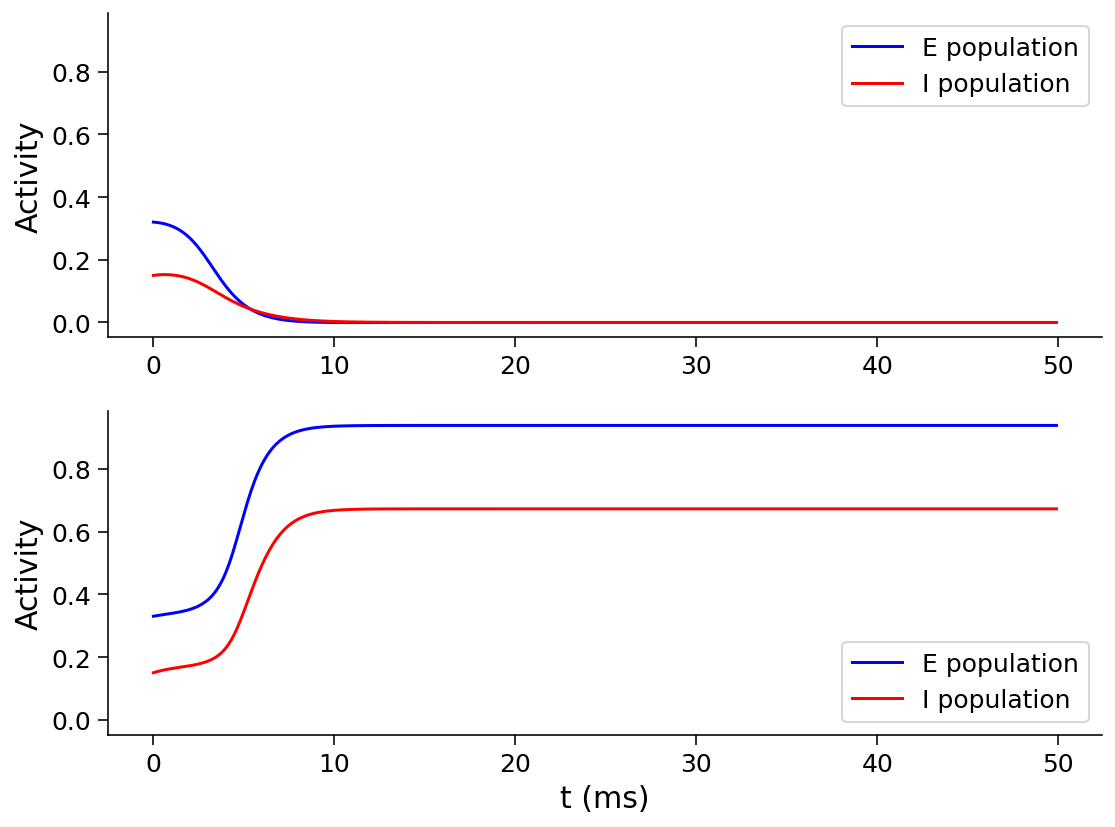
\includegraphics[scale=0.28]{Figures/DN/DN_Figure6.png}
\end{center}
\end{subbox}

\end{textbox}
%%%%%%%%%%%%%%%%%%%%%%%%%%%%%%%%%%%%%%%%%%%%%%%%%%%%%%
%%%%%%%%%%%%%%%%%%%%%%%%%%%%%%%%%%%%%%%%%%%%%%%%%%%%%%
\begin{textbox}{\href{https://compneuro.neuromatch.io/tutorials/W2D4_DynamicNetworks/chapter_title.html}{Wilson-Cowan Model (W2D4T2)} }
\begin{subbox}{subbox}{Phase plane analysis}
\scriptsize
Just like we used a graphical method to study the dynamics of a 1-D system in the previous tutorial, here we will learn a  graphical approach called \textbf{phase plane analysis} to study the dynamics of a 2-D system like the Wilson-Cowan model.

So far, we have plotted the activities of the two populations as a function of time. Instead, we can plot the two activities $r_E(t)$ and $r_I(t)$ against each other at any time point $t$. This characterization in the `rI-rE` plane $(r_I(t), r_E(t))$ is called the \textbf{phase plane}. Each line in the phase plane indicates how both $r_E$ and $r_I$ evolve with time.
\begin{center}
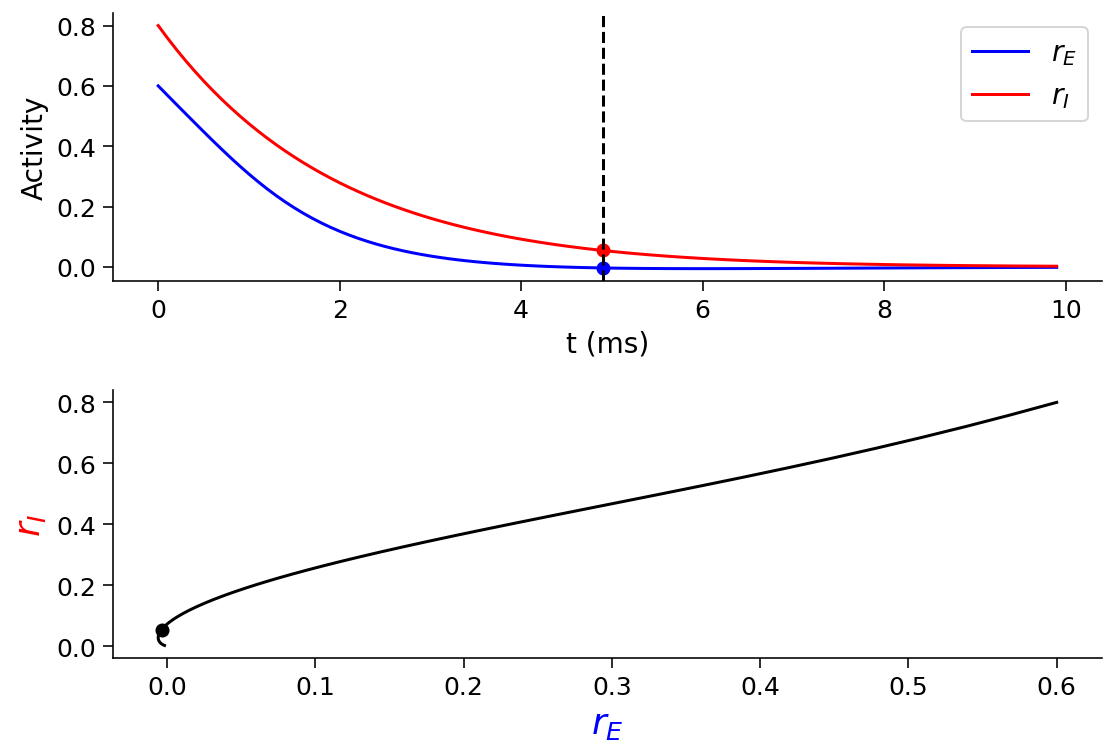
\includegraphics[scale=0.23]{Figures/DN/DN_Figure7.png}
\end{center}
\end{subbox}
\begin{subbox}{subbox}{Nullclines of the Wilson-Cowan Equations
}
\scriptsize
An important concept in the phase plane analysis is the "nullcline" which is defined as the set of points in the phase plane where the activity of one population (but not necessarily the other) does not change.

In other words, the $E$ and $I$ nullclines of Equation $(1)$ are defined as the points where $\displaystyle{\frac{dr_E}{dt}}=0$, for the excitatory nullcline, or $\displaystyle\frac{dr_I}{dt}=0$ for the inhibitory nullcline. That is:

\begin{align*}
-r_E + F_E(w_{EE}r_E -w_{EI}r_I + I^{\text{ext}}_E;a_E,\theta_E) &= 0  \\
-r_I + F_I(w_{IE}r_E -w_{II}r_I + I^{\text{ext}}_I;a_I,\theta_I) &= 0  
\end{align*}
\end{subbox}

\end{textbox}
%%%%%%%%%%%%%%%%%%%%%%%%%%%%%%%%%%%%%%%%%%%%%%%%%%%%%%
%%%%%%%%%%%%%%%%%%%%%%%%%%%%%%%%%%%%%%%%%%%%%%%%%%%%%%
\begin{textbox}{\href{https://compneuro.neuromatch.io/tutorials/W2D4_DynamicNetworks/chapter_title.html}{Wilson-Cowan Model (W2D4T2)} }

\begin{subbox}{subbox}{Compute the nullclines of the Wilson-Cowan model}
\scriptsize
Along the nullcline of excitatory population , you can calculate the inhibitory activity by rewriting it as 

\begin{align*}
r_I = \frac{1}{w_{EI}}\big{[}w_{EE}r_E - F_E^{-1}(r_E; a_E,\theta_E) + I^{\text{ext}}_E \big{]}.
\end{align*}

where $F_E^{-1}(r_E; a_E,\theta_E)$ is the inverse of the excitatory transfer function (defined below). 

Along the nullcline of inhibitory population, you can calculate the excitatory activity by rewriting it as  
\begin{align*}
r_E = \frac{1}{w_{IE}} \big{[} w_{II}r_I + F_I^{-1}(r_I;a_I,\theta_I) - I^{\text{ext}}_I \big{]}  
\end{align*}

where $F_I^{-1}(r_I; a_I,\theta_I)$ is the inverse of the inhibitory transfer function.

The inverse of the sigmoid shaped **f-I** function that we have been using is:

$$
F^{-1}(x; a, \theta) = -\frac{1}{a} \ln \left[ \frac{1}{x + \displaystyle \frac{1}{1+\text{e}^{a\theta}}} - 1 \right] + \theta.
$$
\begin{center}
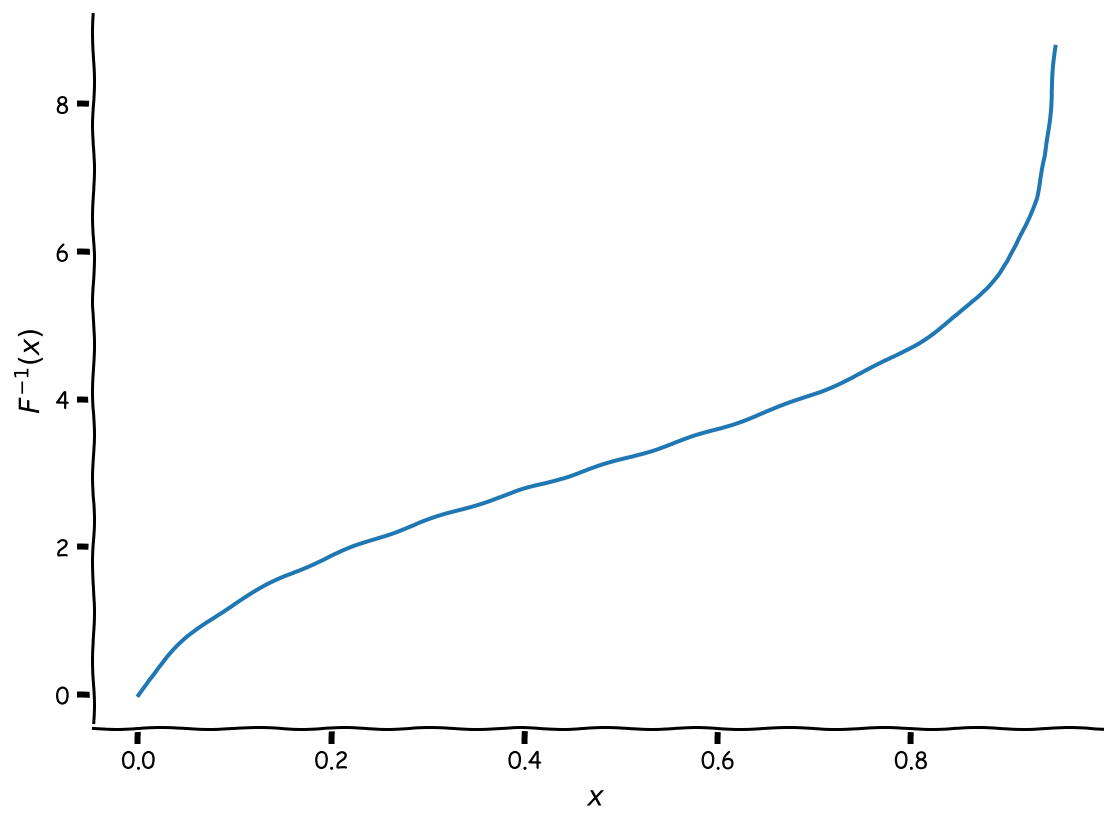
\includegraphics[scale=0.15]{Figures/DN/DN_Figure8.png}
\end{center}
Now you can plot the nullclines
\begin{center}
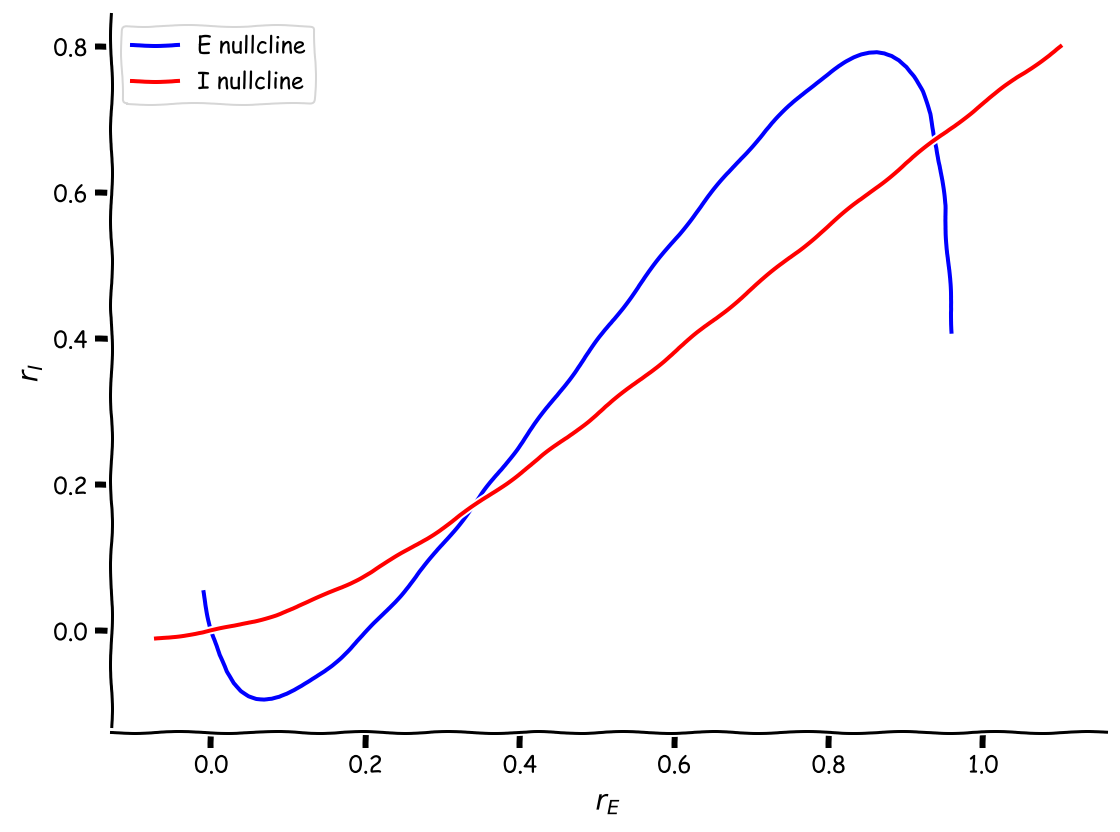
\includegraphics[scale=0.15]{Figures/DN/DN_Figure9.png}
\end{center}

\end{subbox}
\end{textbox}
%%%%%%%%%%%%%%%%%%%%%%%%%%%%%%%%%%%%%%%%%%%%%%%%%%%%%%
%%%%%%%%%%%%%%%%%%%%%%%%%%%%%%%%%%%%%%%%%%%%%%%%%%%%%%
\begin{textbox}{\href{https://compneuro.neuromatch.io/tutorials/W2D4_DynamicNetworks/chapter_title.html}{Wilson-Cowan Model (W2D4T2)} }

\begin{subbox}{subbox}{Vector field}
\scriptsize
How can the phase plane and the nullcline curves help us understand the behavior of the Wilson-Cowan model?

The activities of the $E$ and $I$ populations $r_E(t)$ and $r_I(t)$ at each time point $t$ correspond to a single point in the phase plane, with coordinates $(r_E(t),r_I(t))$. Therefore, the time-dependent trajectory of the system can be described as a continuous curve in the phase plane, and the tangent vector to the trajectory, which is defined as the vector $\bigg{(}\displaystyle{\frac{dr_E(t)}{dt},\frac{dr_I(t)}{dt}}\bigg{)}$, indicates the direction towards which the activity is evolving and how fast is the activity changing along each axis. In fact, for each point $(E,I)$ in the phase plane, we can compute the tangent vector $\bigg{(}\displaystyle{\frac{dr_E}{dt},\frac{dr_I}{dt}}\bigg{)}$, which  indicates the behavior of the system when it traverses that point. 

The map of tangent vectors in the phase plane is called \textbf{vector field}. The behavior of any trajectory in the phase plane is determined by \begin{enumerate}
    \item 
the initial conditions $(r_E(0),r_I(0))$, and 
\item the vector field $\bigg{(}\displaystyle{\frac{dr_E(t)}{dt},\frac{dr_I(t)}{dt}}\bigg{)}$.
\end{enumerate} 
In general, the value of the vector field at a particular point in the phase plane is represented by an arrow. The orientation and the size of the arrow reflect the direction and the norm of the vector, respectively.

To compute and plot the vector field we use
\begin{align*}
\frac{dr_E}{dt} &= [-r_E + F_E(w_{EE}r_E -w_{EI}r_I + I^{\text{ext}}_E;a_E,\theta_E)]\frac{1}{\tau_E}\\
\frac{dr_I}{dt} &= [-r_I + F_I(w_{IE}r_E -w_{II}r_I + I^{\text{ext}}_I;a_I,\theta_I)]\frac{1}{\tau_I}.   
\end{align*}

The phase plane plot below shows us that:

\begin{itemize}
    \item 
 Trajectories seem to follow the direction of the vector field.
\item Different trajectories eventually always reach one of two points depending on the initial conditions.
\item The two points where the trajectories converge are the intersection of the two nullcline curves.
\end{itemize}


\begin{center}
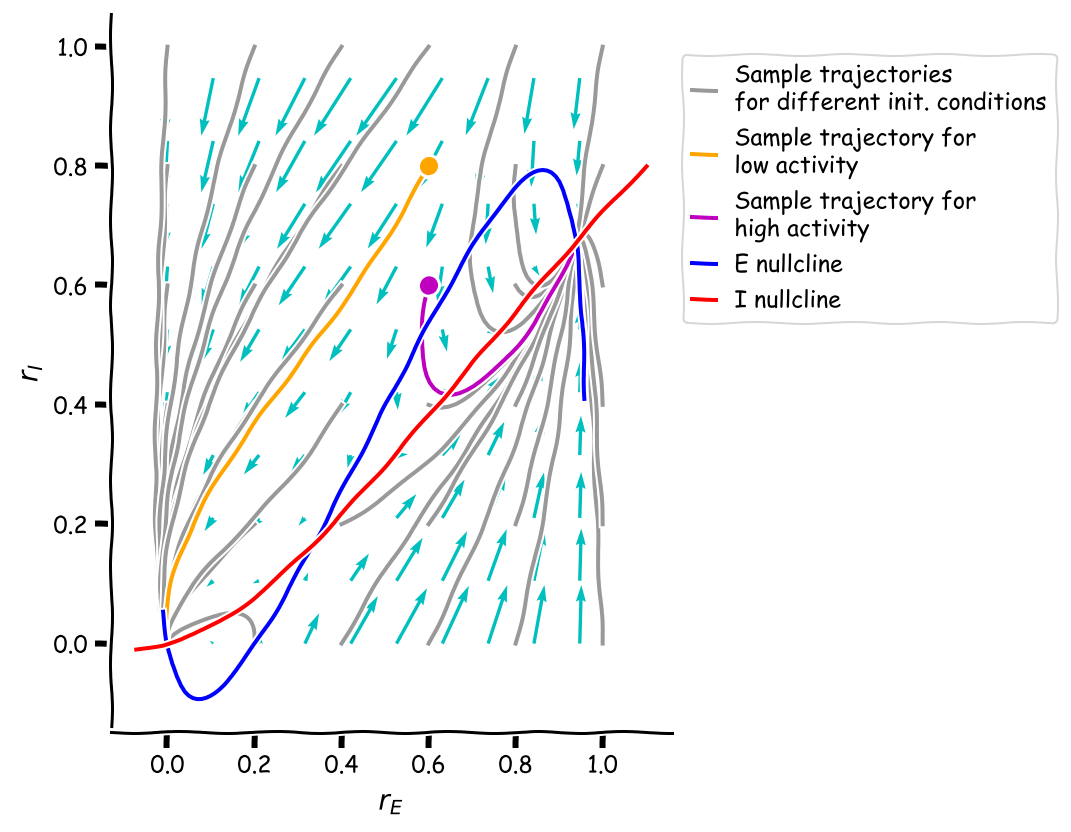
\includegraphics[scale=0.13]{Figures/DN/DN_Figure10.png}
\end{center}

\end{subbox}
\end{textbox}
\end{multicols}

\end{document}
